\chapter{Gene Discovery through Plant Genome Environment Associations:
The Case for Enhanced Machine Learning Models of Soil Phosphorus Availability}
\label{chap-two}

\newrefsection

\section{Abstract}

\section{Background} 

Wild plants and crops show genetic adaptation to local soil conditions. 
In the high end of selection strength, maladapted individuals are not even able to survive extreme environments. 
This is the case of serpentine soils, which are very adverse to plant life, having alkaline pH, limiting amounts of nutrients like phosphorus, and elevated levels of heavy metals like nickel \citep{alexander2006}.
However, some populations of \textit{Mimmulus guttatus} are able to thrive there nonetheless. 
Using 2 independent mapping populations \citep{selby2018} were able to map a Quantitative Trait Locus (QTL) underlying survival in serpentine soils.
Furthermore, with common garden experiments, they isolated the genotypic effect of soil adaptation from water availability, exposure, and community composition \citep{selby2018}.
In less extreme cases, soil selective pressures do not result in death but penalize plant growth and yield.
For example, \citep{lasky2015-ar} found candidate \textit{Sorghum} adaptive loci to acid soils using Genome Environment Associations with topsoil pH in African traditional varieties. 
Later they were able to validate, in an independent \textit{Sorghum bicolor} inbred panel from the USA, the candidate SNPs by assessing their predictive value on seedling root growth in an acid substrate, where they contributed with a low but significant effect (Pearson $r \approx 0.3$) \citep{lasky2015-ar}. 

During domestication, maize has been selected for architectural root traits that increase resource acquisition in comparison to its wild relatives \citep{burton2013a,perkins2021}. When compared with teosinte, traditional Mexican maize varieties have a higher number of seminal roots \citep{burton2013a}, and this phenotype shows a pattern of local adaptation correlated with mean annual precipitation, and consequently to drought \citep{mclaughlin2023}.
Given the continuous selection for yield in industrial agriculture, optimal conditions for crops are rarely met in natural soils, and elite corn hybrids usually require fertilizer and other artificial inputs for maximal output. 

Low soil phosphorus availability for crops is the rule rather than the exception at the global scale \citep{mcdowell2023,batjes2019,lyons2023}. 
And Mexican soils are no different. 
I calculate a median topsoil available phosphorus concentration of 3.5 ppm (mg/kg) with 79\% of the natural soils samples below 10 ppm \citep{paz-pellat2018} \autoref{fig::obeserved_PHOS} (see Methods). 
For comparison, the minimal US test phosphorus recommendations for corn start at 15 ppm \citep{lyons2023}.

Soil tests cannot precisely tell the exact available amount of phosphorus for plants, instead, they provide an estimate of what the plant might acquire \citep{beegle2002}. 
These estimations are based on extensive yield trials at a range of soil phosphorus test values in multiple types of soils, which allows the construction of calibration curves and the assessment of critical values with the ultimate goal of giving farmers valid practical recommendations at the local level\citep{culman2023, dodd2005, beegle2002}. 
The most common extractants for phosphorus tests are Bray-1 (aka Bray-Kurtz)\citep{bray1945}, Meilich-3 \citep{mehlich1984} and Olsen \citep{olsen1954}.
The first two work best for neutral and acid soils and the last one correlates better with plant yield in alkaline calcareous soils \citep{culman2020}.
Due to differences in soils and policies between states, there is no single standard for soil phosphorus tests in the US \citep{lyons2023}.
The minimum soil test phosphorus recommendations for crop optimal yield in the USA, vary between 15 to 31 ppm depending on test and state \citep{lyons2023}, with yield trials of 10 ppm Bray-1 phosphorus producing relative yield losses up to 50\% \citep{dodd2005}. In contrast to the US, the Mexican government has adopted a straightforward approach. 
The reported available phosphorus for \citep{paz-pellat2018}, hereafter referred to as PHOS, corresponds to Bray-1 test phosphorus for neutral and acid soils (aka Bray-Kurtz)\citep{bray1945} and to Olsen test phosphorus for basic soils \citep{olsen1954}.

However, I find that global models of plant-available phosphorus, and other phosphorus parameters, have a very low prediction value in Mexico, with the Pearson correlation between these experimental \citep{paz-pellat2018} and the predicted values below $r=0.1$ \autoref{fig::phoscorrelation}.

For this reason, I use digital soil mapping based on machine learning techniques to predict the distribution of plant soil available phosphorus

\begin{figure}[!ht]
\centering
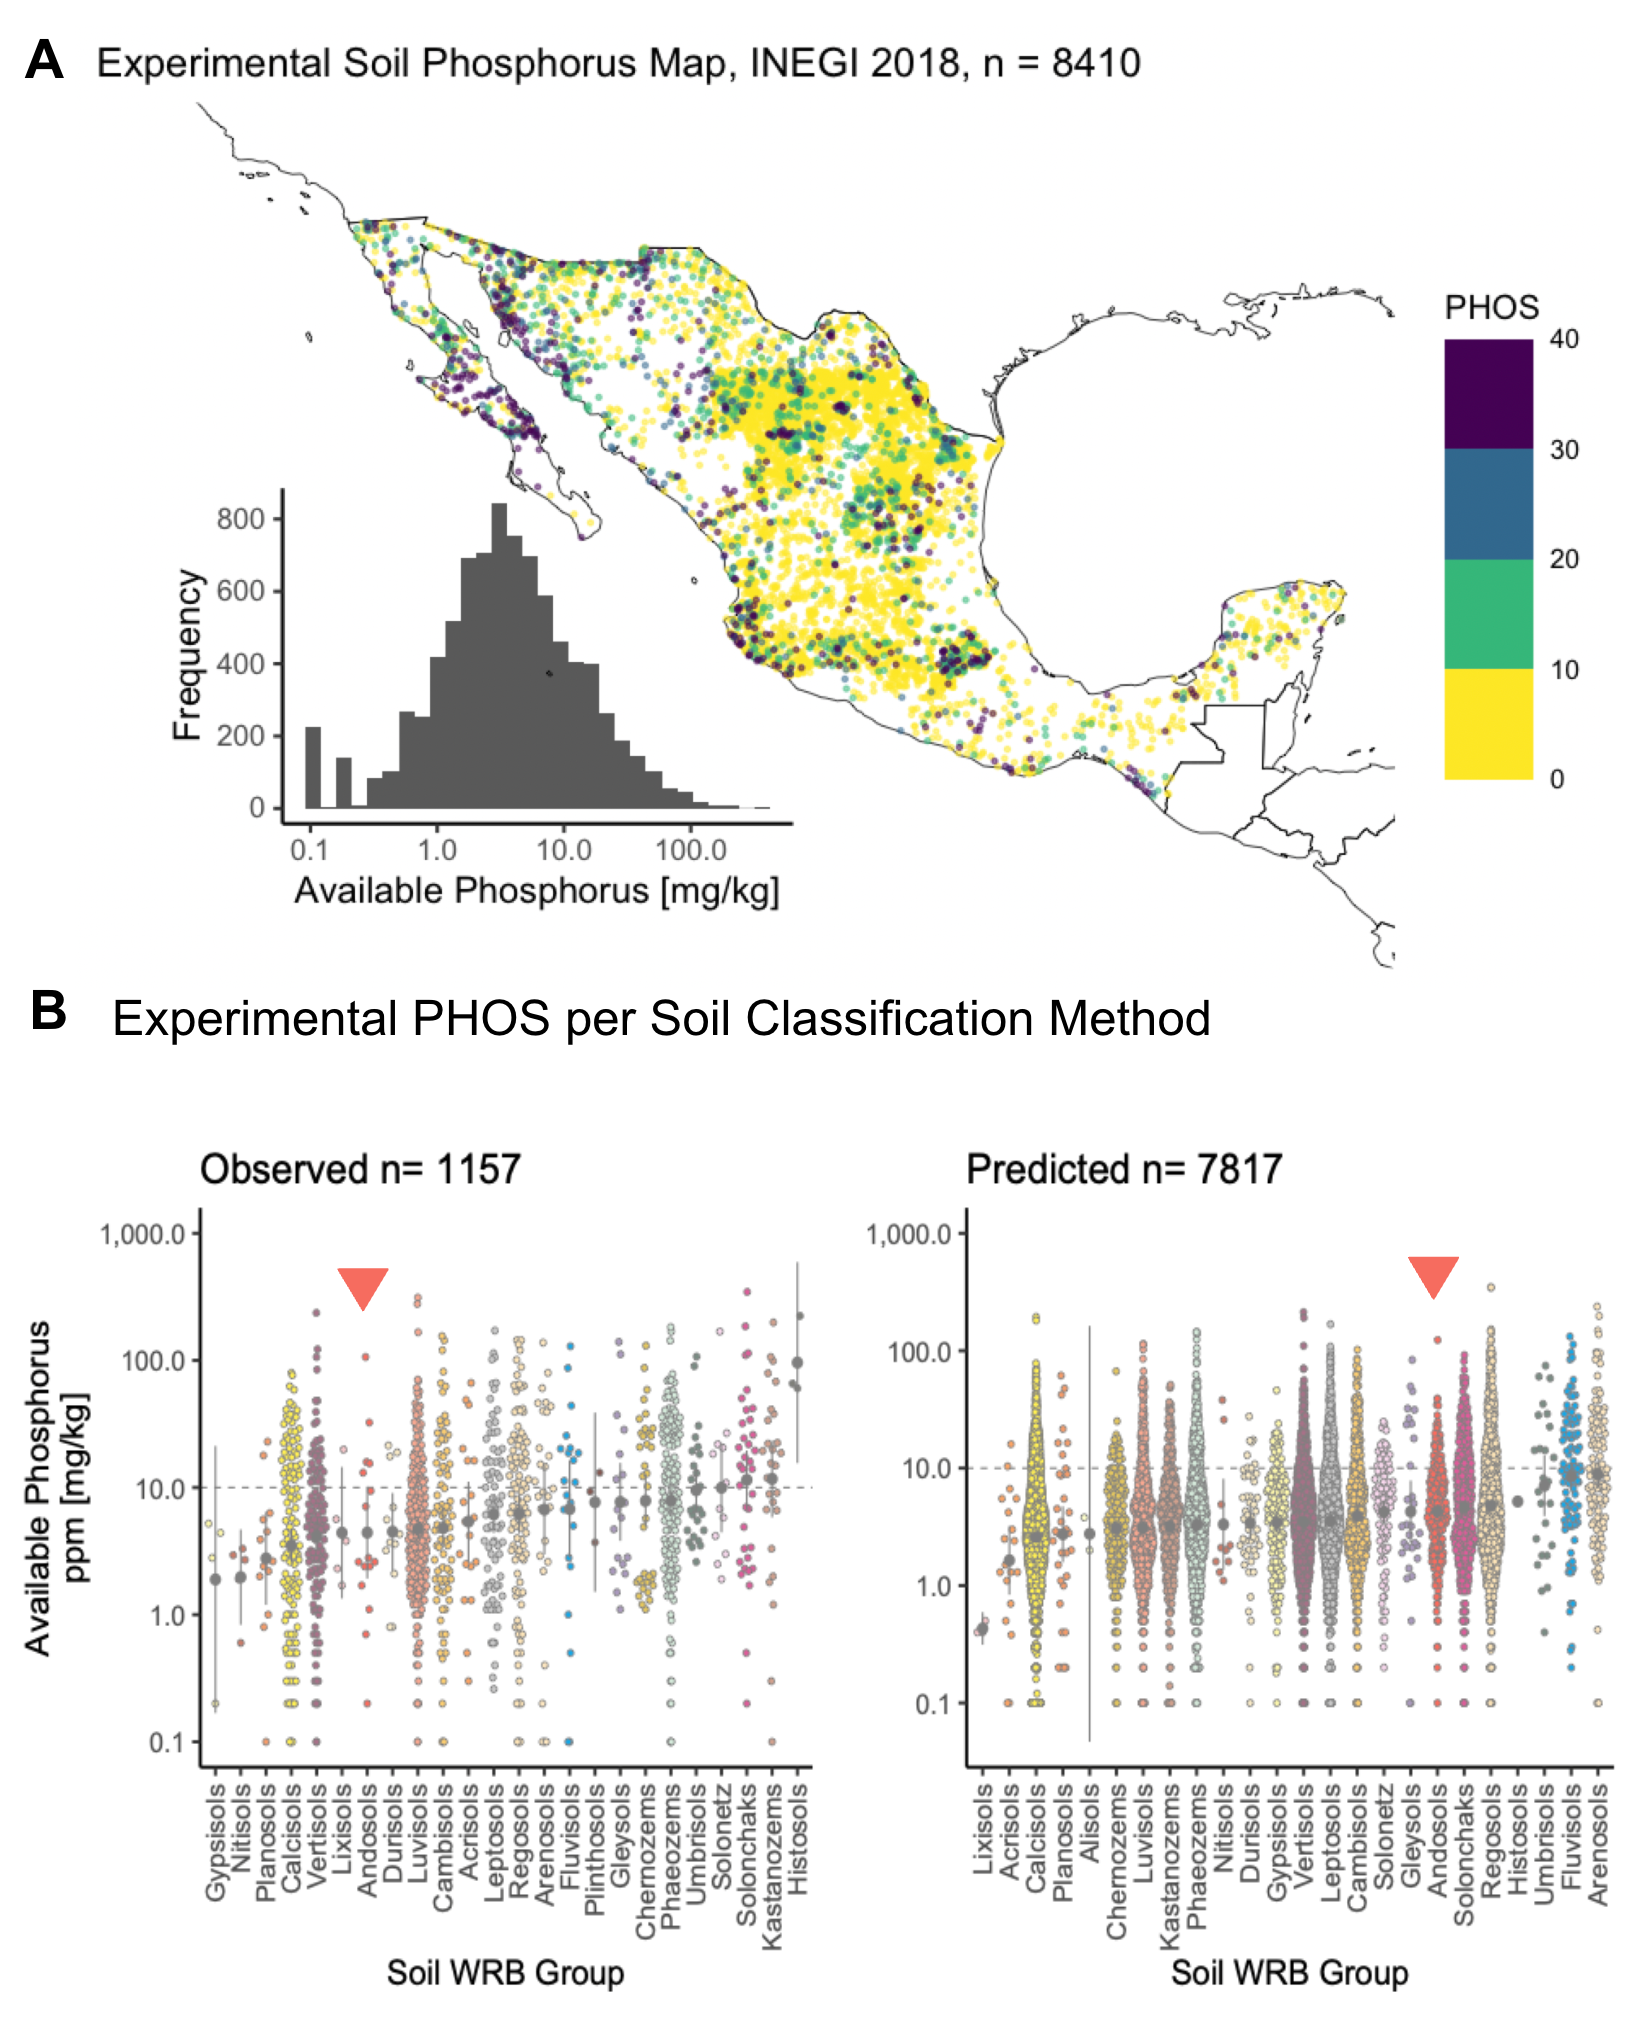
\includegraphics[width=0.9\linewidth]{Chapter-2/figs/obeserved_PHOS.png}
\caption[Experimental values for topsoil plant available phosphorus (PHOS) in Mexico]{\textit{\textbf{Experimental values for topsoil plant available phosphorus (PHOS) in Mexico.}} \\\hspace{\textwidth} 
\textbf{(A)} Geographical distribution of sampled soil profiles. For acid and neutral soils ($\text{pH} \leq 7$) the reported PHOS value corresponds to Bray-1 phosphorus. For basic soils Olsen phosphorus is reported as PHOS  \citep{paz-pellat2018}.
\textbf{(B)} Available phosphorus per WRB soil group determination method, \textit{left:} observed WRB determination in the field for INEGI reference profiles, \textit{right:} assignation of dominant soil in the corresponding map unit (polygon) in \citep{inegi2013}. The downward triangle points to Andosol group soils}
\label{fig::obeserved_PHOS}
\end{figure}
\clearpage

 
%% \begin{figure}[!ht]
%% \centering
%% 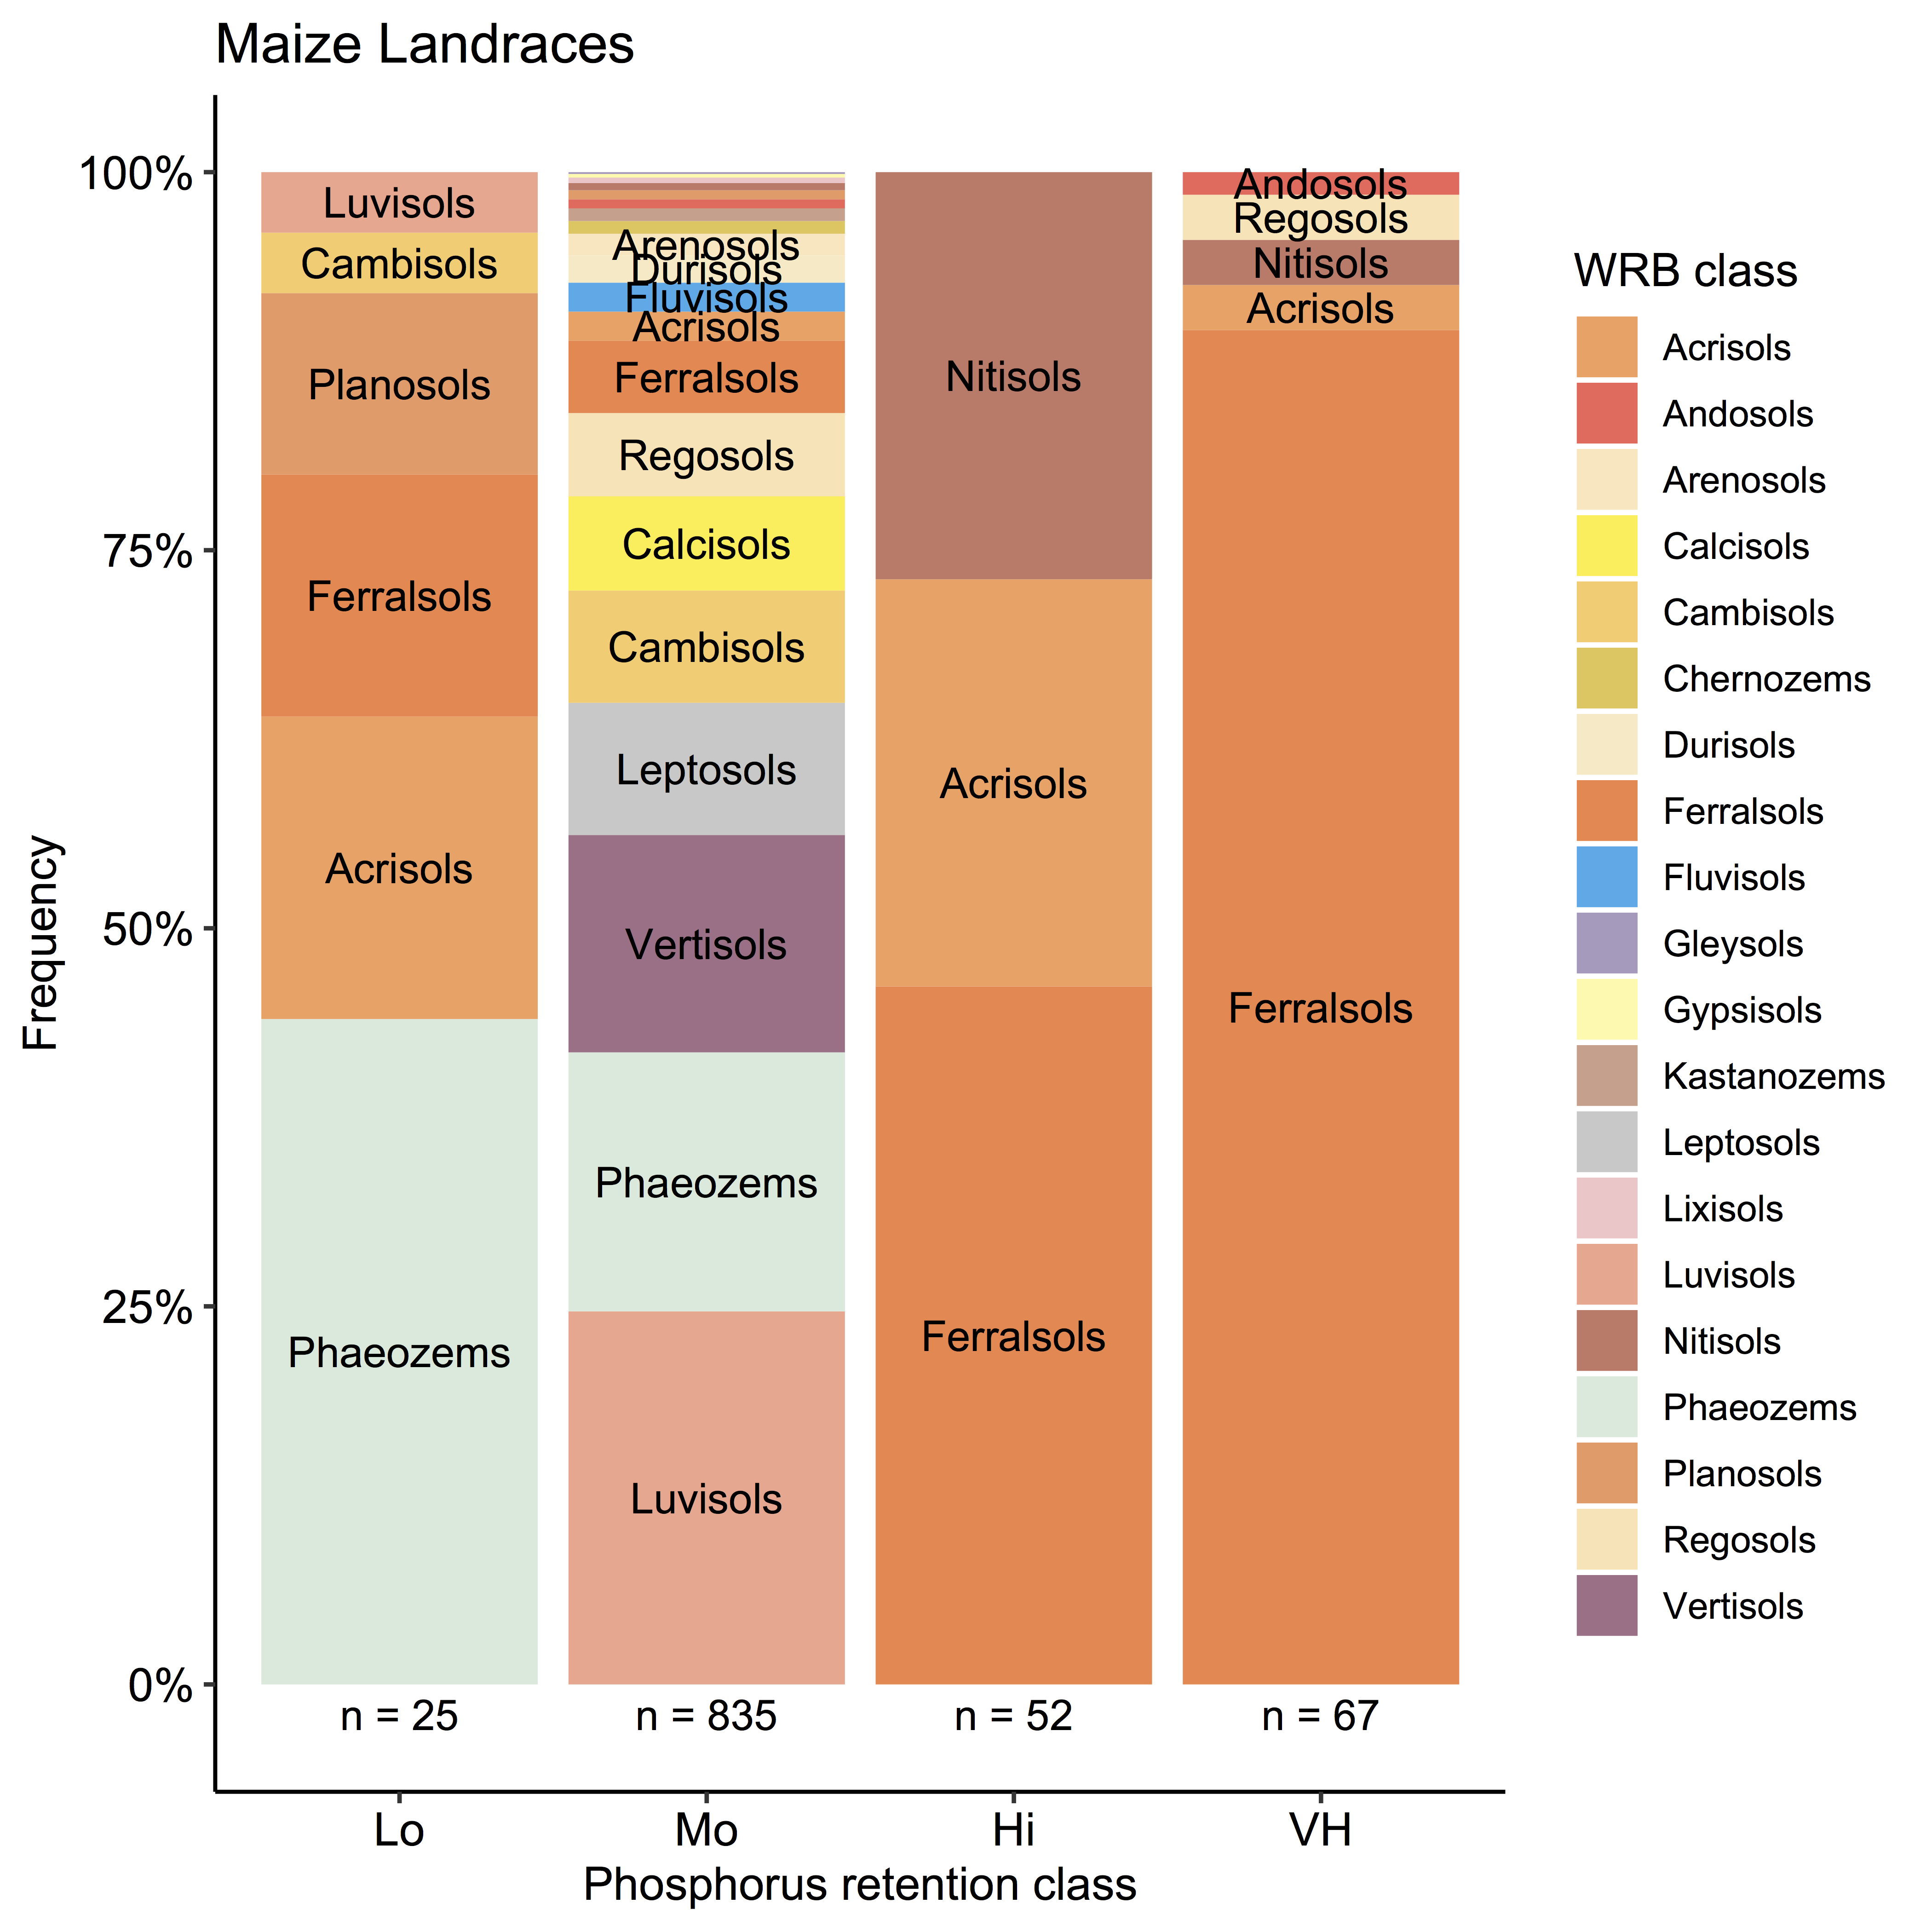
\includegraphics[width=\linewidth]{Chapter-2/figs/WRB_Pret.png}
%% \caption[Phosphorus Retention Potential For Maize Traditional Varieties in Latin America and the Caribbean]{\textbf{\textit{Phosphorus Retention Potential For Maize Traditional Varieties in Latin America and the Caribbean.}}
%% Based on \citep{batjes2011}.  Each soil unit corresponds to a mineral descriptor, e.g. Acrisol soil units can be gleyic, humic, orthic, or plinthic. Ferric acrisols have very low phosphorus solubility potential (first column), the other three acrisol units have low solubility (second column). The soil groups with predominantly High and Very High solubility are Ferralsols, Andosols, Acrisols, and Nitosols.}
%% \label{fig::WRB_Pret}
%% \end{figure}
%% \clearpage

\section{Methods}
\subsection{Building and Validating a Model for Plant Available Phosphorus Distribution in Mexico}

To find associations between plant-available soil phosphorus and the genetic diversity of maize traditional varieties, I started by compiling public datasets on global phosphorus distribution. 
Because of its high resolution and interpretability, I intended to use the Olsen \citep{olsen1954} phosphorus predictions by \citep{mcdowell2023}.
However, the training data for this model contained no experimental Olsen determinations for Mexico, just 32 data points regressed from Bray-1 or resin values. 

In addition to \citep{mcdowell2023}, I searched for other datasets and parameters that could be correlated to experimental measures of plant-available phosphorus in soils. These included total phosphorus from \citep{hexianjin2022}, labile and total phosphorus from \citep{yang2013}, phosphorus by Bray-1, Olsen and Mehlich \citep{mehlich1984} methods, New Zealand phosphorus retention from \citep{shangguan2014} and NP limitation from \citep{du2020}.

Knowing that these models relied on a poor sampling Latin America, I decided to use as a benchmark the published experimental phosphorus data from the Instituto Nacional de Estadística y Geografía \citep{paz-pellat2018} of georeferenced soil profiles collected between 1969 to 2006.
This set contained topsoil phosphorus measurements as extractable phosphorus concentration in ppm [mg/kg] for 13092 gelolocalized soil profiles, divided into 8325 datapoints for  Olsen phosphorus (soils $\text{pH} > 7$) and 4767 data points for Bray phosphorus  (soils with $\text{pH} \leq 7$) for Mexico. 

For investigating the phosphorus distribution among different soil types according to WRB taxonomy \citep{wrb2014},  I used the field determinations of WRB soil group for the INEGI Serie II data \citep{inegi2013} and corresponding interpretation \citep{inegi2011,inegi2009} that matched both in profile identifier and geolocation within a 150m error. 

Then I followed the random forest based methodology for soil predictive mapping developed by \citep{hexianjin2022} because of its demonstrated prediction value for total phosphorus, interpretability and computational time savings in comparison with the more onerous 150 input predictor models of \citep{hengl2019} or \citep{mcdowell2023}. 
Here I used the maps for 16 predictors of available phosphorus, improving data cleanup and resolution where possible.
The predictors were as follows: Mean Annual Temperature and Mean Annual Precipitation from BioClim 2.0 at 10 km resolution \citep{fick2017}; WRB soil groups at 10 km and pH, soil organic carbon, bulk density at 250 m resolution, from SoilGrids 250 \citep{hengl2019,hengl2017,wrb2022,scheffe2015}, USDA taxonomy order from OpenLandMap at 250 m, biomes fom Resolve Ecoregions \citep{dinerstein2017} at 10 km, Mean Annual Net Primary Production from MODIS \citep{running2015a} at 250 m, elevation at 15m resolution from INEGI CEM 3.0 \citep{inegi2019}, slope at 1 km from EarthEnv \citep{amatulli2018}, soil depth at 10 km from Land-Atmosphere Interaction Research Group \citep{shangguan2017}, and lithology from GLiM rasterized at 10 km resolution\citep{hartmann2012}.
% (details on Supplementary file S1).
All coordinates were matched to WGS84 latitude longitude for extraction of values from each raster using the custom R scripts.

I ran 15 simple random forest models with these 16 predictors and a single response variable using the R library `randomForest` \citep{liaw2002}. 
I used as output a synthetic variable I called PHOS consisting in the union of those two sets of observations, i.e. the PHOS parameter is a measure of phosphorus availability in the soil that corresponds to Bray I extractable phosphorus if the soil $\text{pH} \leq 7$ and to the Olsen extractable phosphorus if the soil $\text{pH} > 7$. 
I followed the code used by \citep{hexianjin2022}  with 3 random variables selected at each decision node, 500 trees per model, $70\%$ training, $30\%$ testing data a 5-fold cross-validation at each step.
The predictive value of the model is measured as the Pearson correlation between the observed experimental values of available phosphorus concentration and the prediction from the random forest in the test data. 
Cross-validation was used to measure the contribution of each predictor to the model by removing it from the model and measuring the resulting change in the mean standard error of the prediction as a percentage. 
Additionally, I ran an ensemble model based on the 15 outputs of the simple random forest model to see if it would increase predictive values in the test data.

Although I increased the correlation between observations and predictions using the ensemble model up to 0.99, I did not observe an improvement in the test predictions worthy of the more complicated model.

% The POINTDATA needed additional matching in resolution and projection for making a raster prediction at 10 km resolution. So in  I used  \href{https://github.com/sawers-rellan-labs/grassGEA}{a series of custom $`R`$ language scripts} based on the `raster`, `gdal`, `sp` and `stars` libraries for obtaining 15 10km ($0.8883 \times 0.9993$ decimal degrees) latitude longitude WGS84 rasters. This dataset will be referred as MAPDATA.

\subsection{Gene Environment Association}
I used 495,755 SNPs genotyped in 2182 georeferenced maize traditional varieties \citep{romero_navarro2017-cn} to make genome environment associations with the PHOS parameter.
With these, I used a linear mixed model correcting for 10 principal components of the kinship matrix as correction for population structure as fixed effects, in addition to using the kinship matrix itself in the random effects with GEMMA (version: 0.98.3) \citep{vogt2022} as executed by vcf2gwas software (version: 0.8.7) \citep{zhou2012}. Bonforren correction was use to establish the statistical significance threshold.

For comparison, I calculated the fixation index $F_st$ between the deciles at the end of PHOS distribution. 

\section{Results}

\subsection{Random Forest Model of Olsen and Bray Phosphorus Improves Accuracy of Soil Available Phosphorus Estimation in  Mexico}
After building on the work of \citep{hexianjin2022} and \citep{mcdowell2023}, I increased the predictive value of the soil mapping models for Olsen and Bray extractable phosphorus in  Mexico. The the Pearson correlation $r$ from 0.08 to 0.37 (0 and 0.14 $R^2$) for observed and predicted values of plant available phosphorus (PHOS) compared to \citep{mcdowell2023}. PHOS prediction value is well bellow those used for species distributio models, like  mean annual temperature,$R^2$ = 0.98 \citep{fick2017}).
However, our model improves prediction for in Mexico compared to previous global models \cite{mcdowell2023} and a comparable model of plant available phosphorus in  Africa $R^2$ = 0.12  \citep{hengl2017a} 
Appart from the predictive value,  the relative importance of predictors in our models is congruent with the chemical understanding of how phosphorus goes into soil solution.
Phosphorus in solution depends on pH and soil mineralogy, while the total amount of phosphorus in non-fertilized soils should depend mostly on parent material and organic mater fractions.
Thus the random forest predictor importance as measured by \%IncMSE in our small model is easier to understand than models including multiple multispectral vegetation indices and climate variables \citep{mcdowell2023}.
This leads us to conclude that we have a more parsimonious model that has better prediction value and better interpretability.

% In addition to this we see good overlap with the training data set for both Africa and LAC (Figure 1C) (MANOVA test), which allows us to make reasonable interpolations. A similar approach increased the total phosphorus predictive value as well from 0.81 to 0.91 (0.65 and 0.81 $R^2$), marginally improving previously reported data for Africa \citep{hengl2017a}, where we expect even less over-fit because of the better sampling and increased mixing of data points in the predictor space.

% Not only our model shows acceptable and improved internal consistency, but it has increased correlations with other reported measurements of available P. For example for the LAC pixels corresponding to the Hou sampling of Hedley available phosphorus the correlation between our Olsen is 0.5  and Bray is 0.4. For the Africa isDASOIL \citep{miller2021b} extractable phosphorus is 0.4.
% At the level of continental and global models our Bray and Olsen predictions have high correlation with McDowell Olsen at the global scale but not in the southern hemisphere, with the predicted water soluble phosphorus in Africa \citep{miller2021b,hengl2017a}and low correlations with previous raster values based on heuristics models like \cite{shangguan2014}, \cite{yang2013} and\cite{batjes2011} retention probabilities.


\begin{figure}[!ht]
\centering
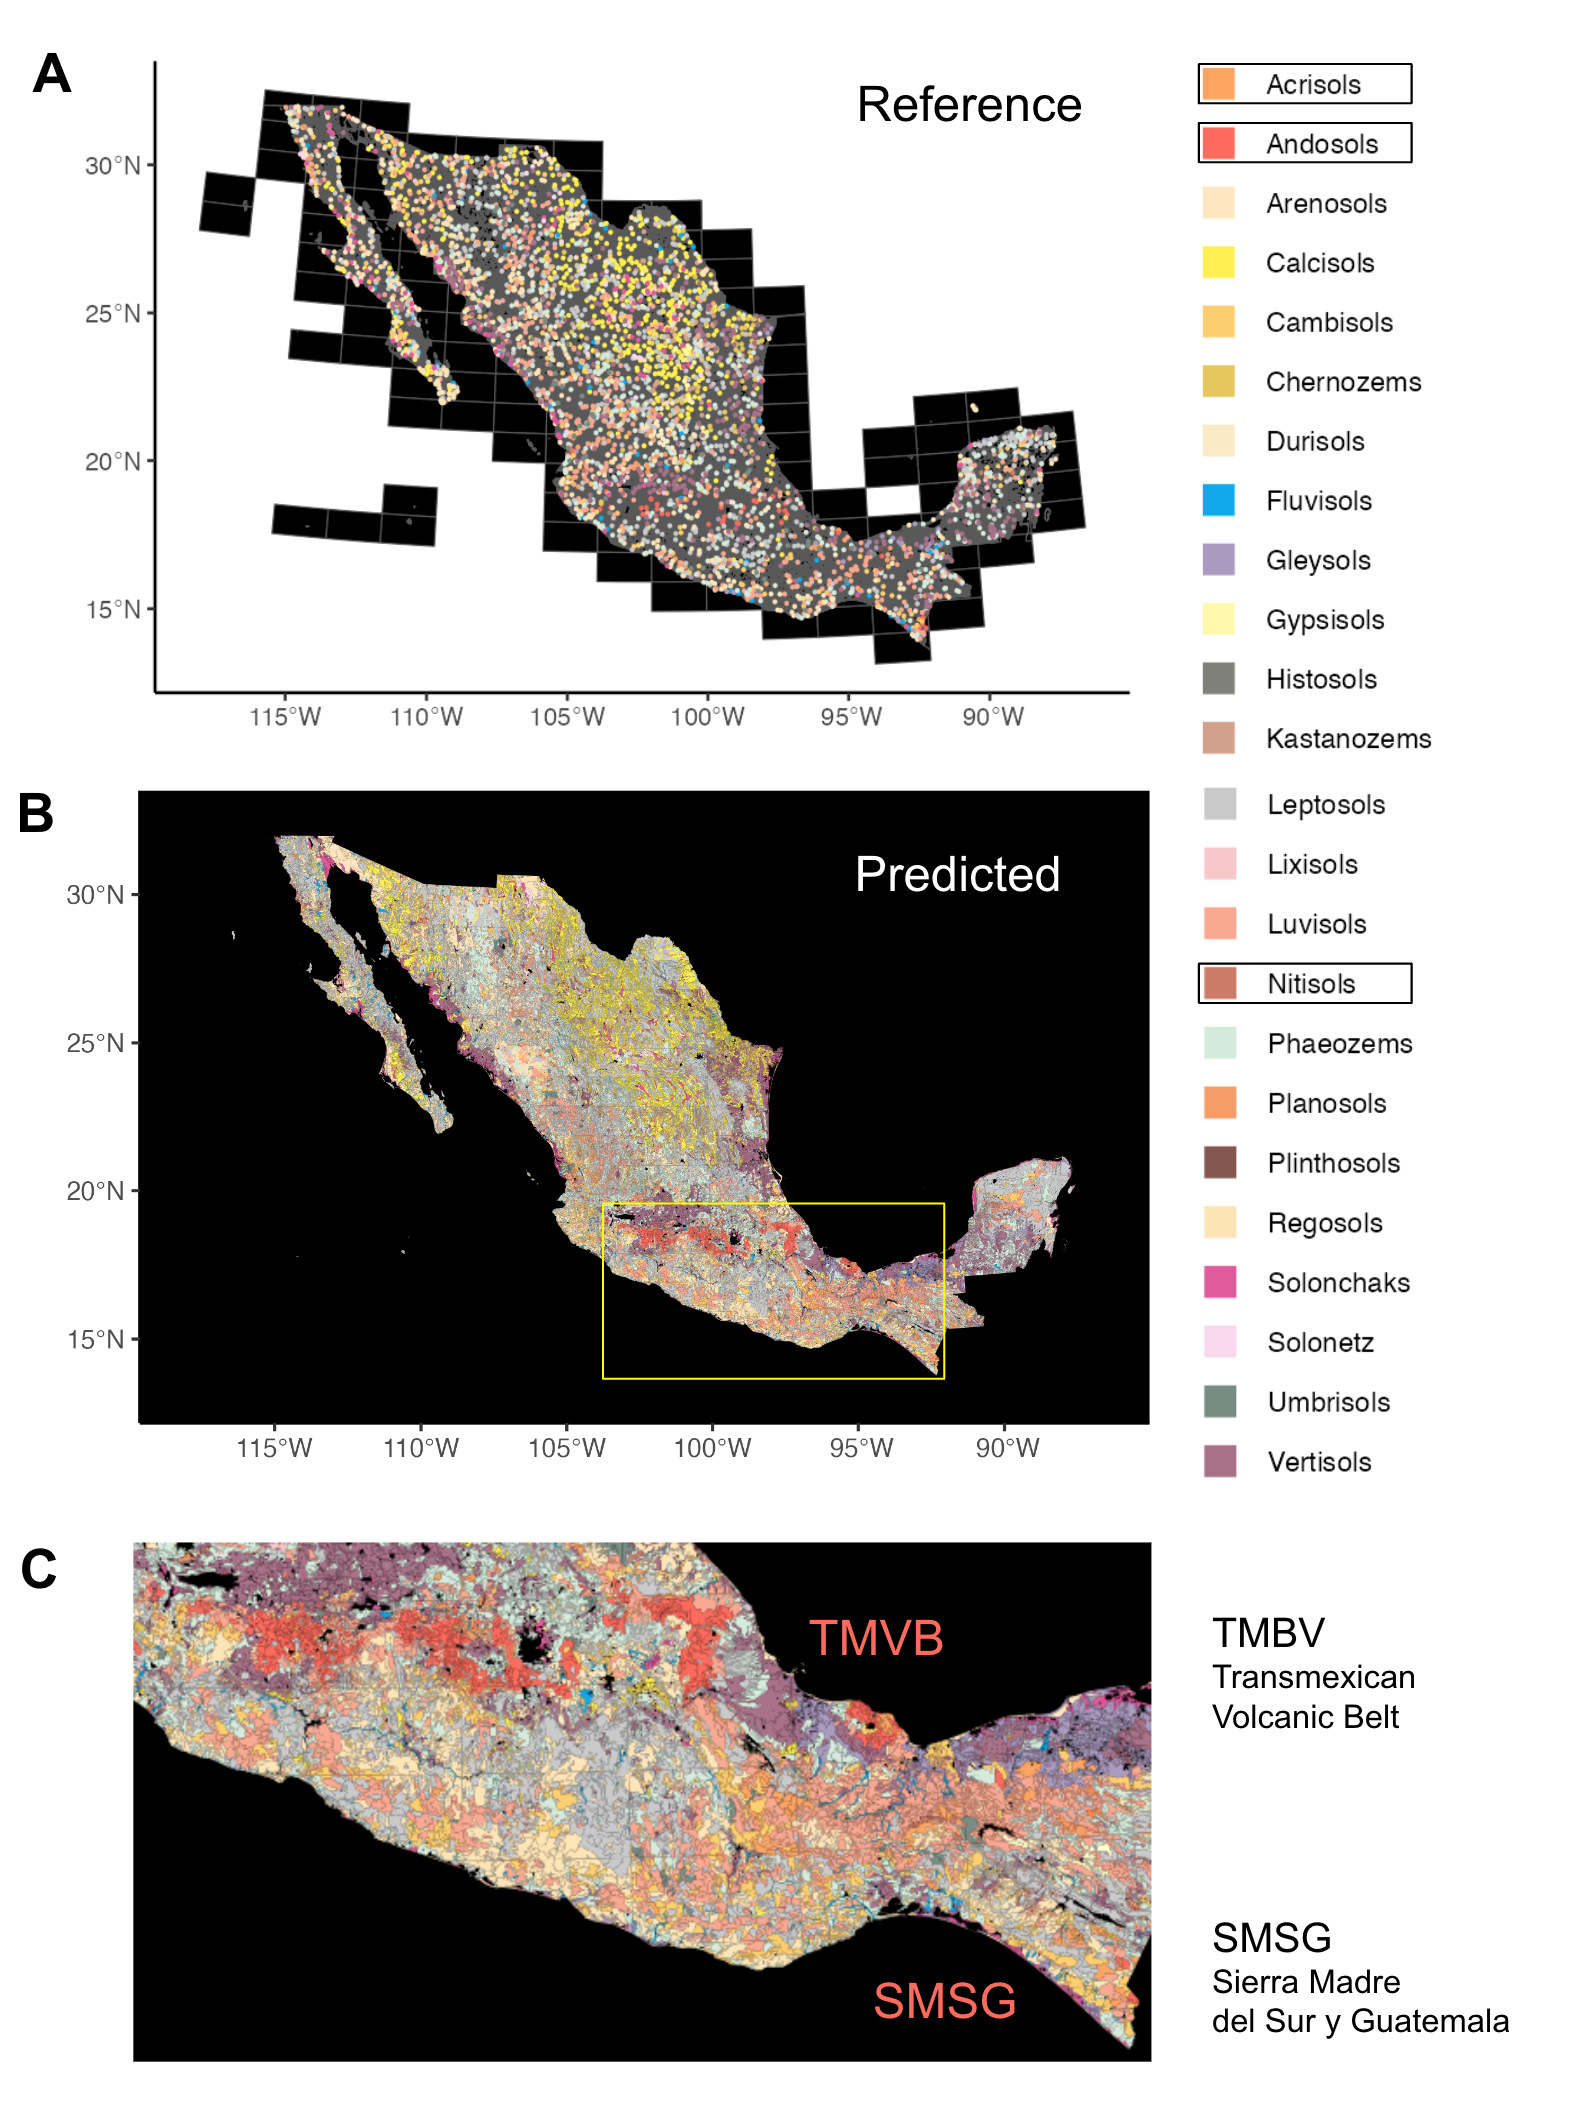
\includegraphics[width=0.9\linewidth]{Chapter-2/figs/WRB_inegi2013map.png}
\caption[WRB Soil Group Classification for Mexican soils according to INEGI]{\textit{\textbf{WRB Soil Group Classification for Mexican soils according to INEGI.}} \\\hspace{\textwidth}
\textbf{(A)} Reference soil profiles ($n \approx 4000$) \citep{inegi2013}.
\textbf{(B)} 1:250000 map prediction for the dominant WRB soil group \citep{inegi2015}
\textbf{(C)} Andosols predominate in the Transmexican Volcanic Belt at high altitudes and are frequent in the Sierra Nevada de Chiapas y Guatemala, collection areas for the Andosol Introgression Resource population \autoref{chap-four}}
\label{fig::WRB_inegi2013map}
\end{figure}
\clearpage


\begin{figure}[!ht]
\centering
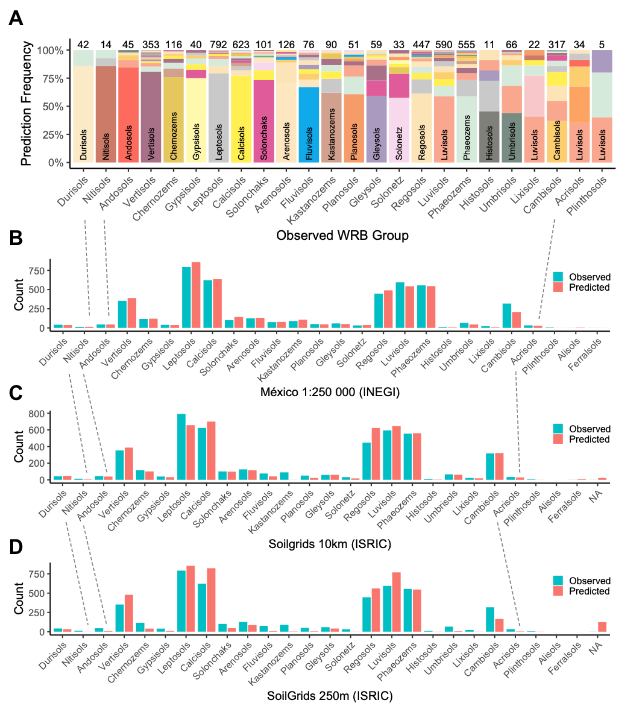
\includegraphics[width=\linewidth]{Chapter-2/figs/WRB_inegi_soilgrids.png}
\caption[Comparison between INEGI and SoilGrids WRB soil Classification Maps]{\textit{\textbf{Comparison between INEGI and SoilGrids WRB soil Classification maps.}} \\\hspace{\textwidth}
\textbf{(A)} INEGI 1:250000 map dominant soil prediction sorted by AUROC, total count above the bar. From Histosols to the right misclassifications are more common than correct classifications. For Lixisisols, Cambisols, Acrisols and Plinthosols the most frequent prediction does not match the observed soil group.
\textbf{(B)}  INEGI 1:250000 map dominant soil prediction in absolute frequency scale (count), same as the number of top of A bars.
\textbf{(C)} Soilgrids 10 km WRB dominant soil prediction. Downscaled resolution from 250 m.
\textbf{(D)} Soilgrids 250 WRB dominant soil prediction, it  has more missing data and underpredicts Andosols}
\label{fig::WRB_inegi_soilgrids}
\end{figure}
\clearpage


\begin{figure}[!ht]
\centering
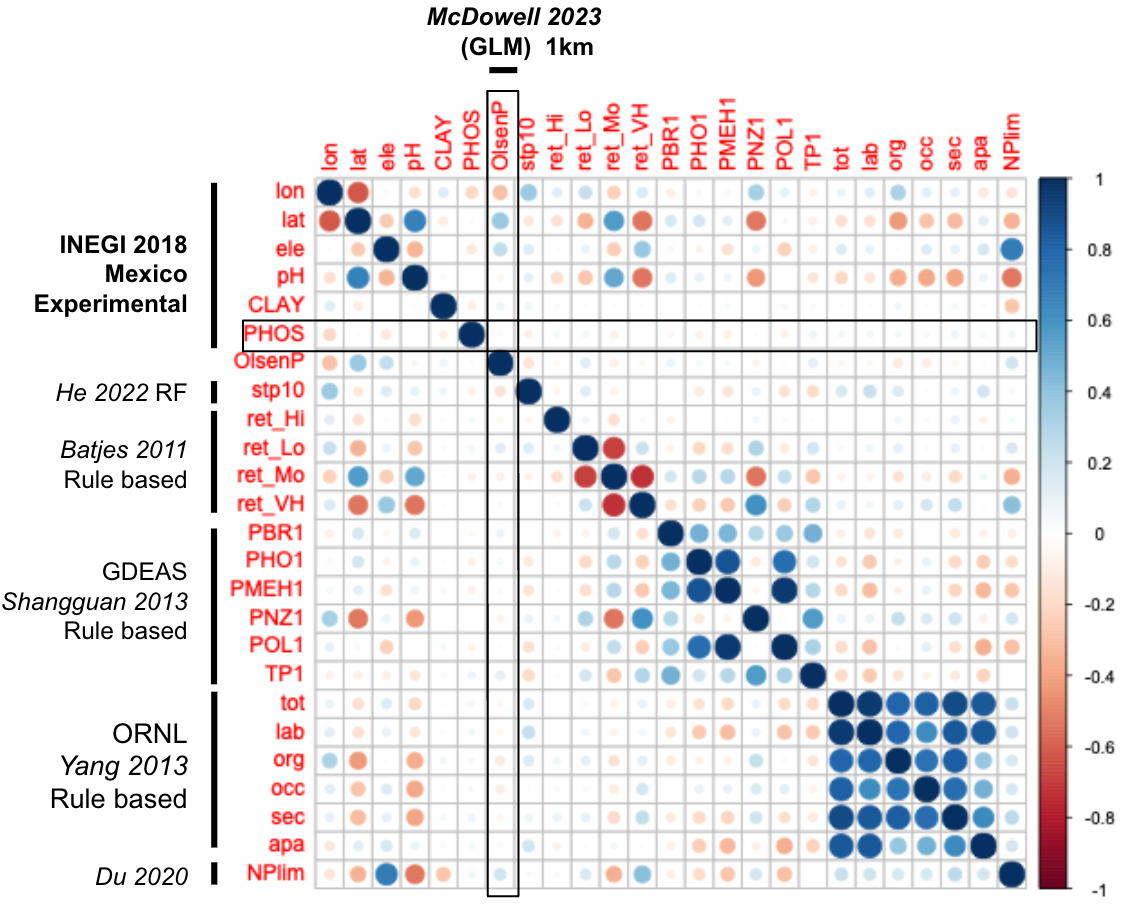
\includegraphics[width=0.65\paperwidth]{Chapter-2/figs/PHOS_correlation.png}
\caption[Pearson correlations (r) between experimental soil available phosphorus in Mexico (PHOS) and predicted phosphorus parameters from global models]{\textit{\textbf{Pearson correlations (r) between experimental soil available phosphorus in Mexico (PHOS) and predicted phosphorus parameters from global models.}} Observed values for lon : longitude, lat: latitude, ele: elevation in \citep{inegi2013}, and clay: clay content, pH, and PHOS: plant available phosphorus in \citep{inegi2013}. Predicted probabilities for Lo: Low, Mo: Moderate, Hi: High, and VH: very high phosphorus retention potential soil classes according to \citep{batjes2011}; predicted
stp10: total phosphorus from \citep{hexianjin2022}, lab: labile and tot: total phosphorus from \citep{yang2013}, phosphorus by Bray, Olsen and Mehlich methods and New Zealand phosphorus retention  from \citep{shangguan2014}; and predicted NPlim: Nitrogen Phosphorus limitation from \citep{du2020}. } 
\label{fig::phoscorrelation}
\end{figure}
\clearpage

\begin{figure}[!ht]
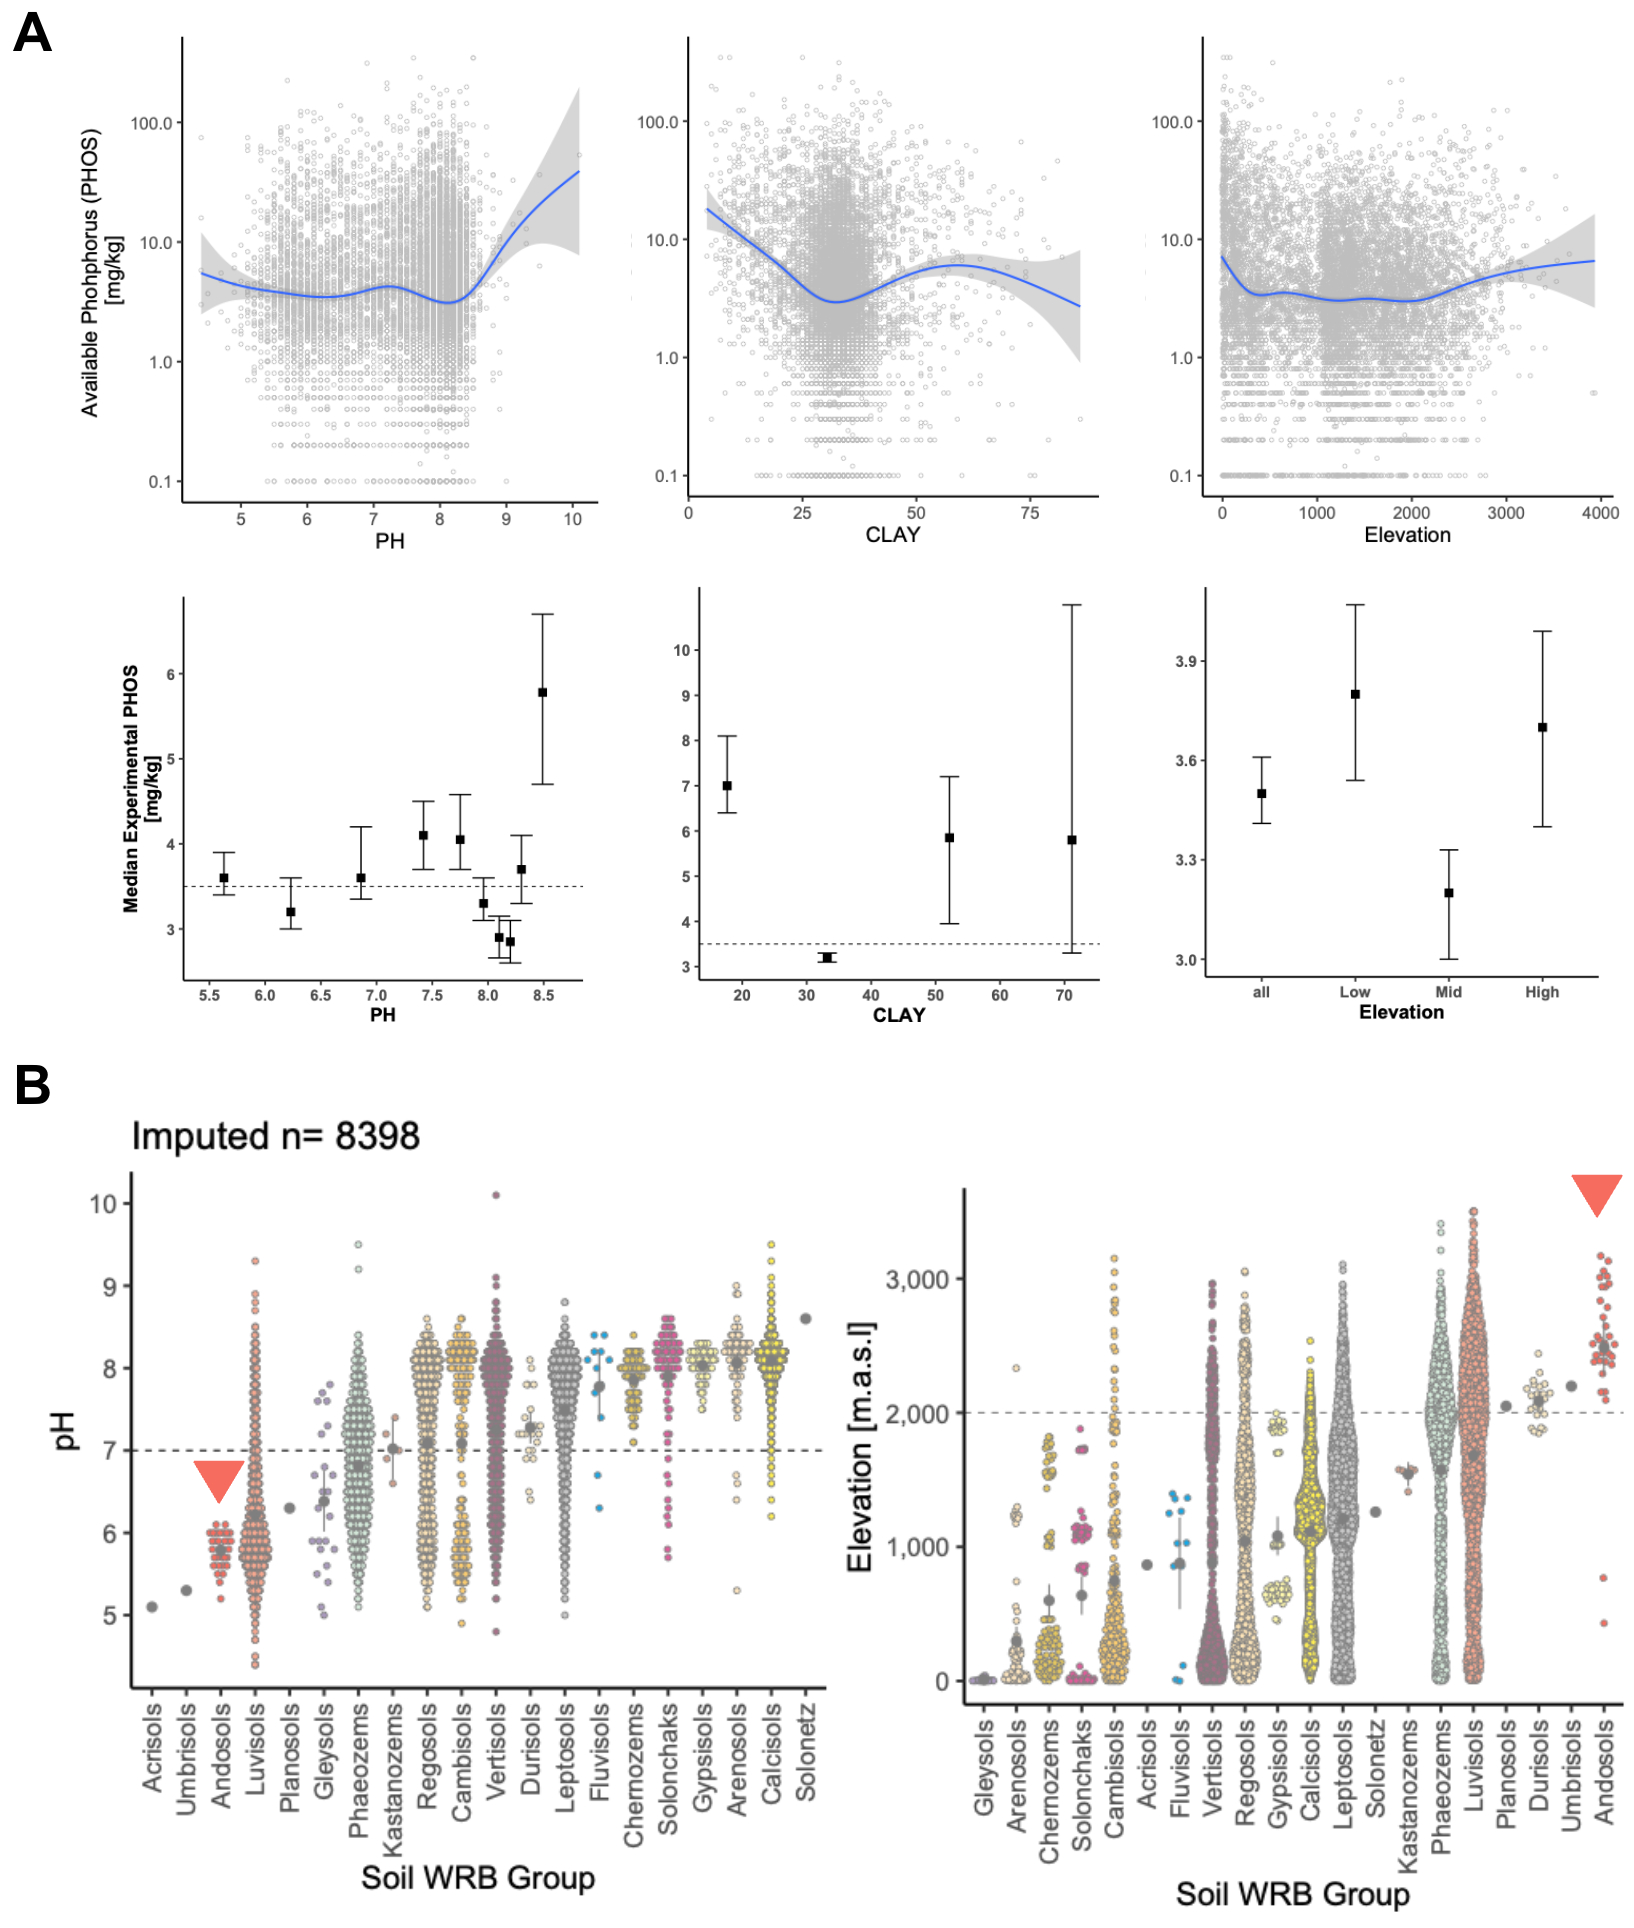
\includegraphics[width=0.9\linewidth]{Chapter-2/figs/marginal_dependencies.png}
\caption[Marginal Dependencies of PHOS. Distribution of pH and elevation by  WRB soil groups] {\textit{\textbf{Marginal Dependencies of PHOS. Distribution of pH and elevation by  WRB soil groups.}} \textbf{(A)} \textit{Top:} Grey circles: experimental values for natural Mexican soils. Spline tendency in blue with confidence interval in grey.  A local maximum of predicted PHOS is found at $\text{pH} = 7.25$, while the global maximum is found at $\text{pH}> 9$. There is a tendency of decreased PHOS with clay content (\%), and there is an increase of PHOS at elevations $> 3000$ masl.
\textit{Bottom:} Zoom on median values, for predictor deciles and 1000 bootstrap confidence intervals. Dashed line is the median value for all samples.
\textbf{(B)} Distribution of pH and elevation by imputed WRB  soil
groups. 
Imputed WRB samples are the union of experimental reference WRB taxonomy determinations, and predictions of dominant soil group from \citep{inegi2013} (see \autoref{fig::obeserved_PHOS} B).
Andosols are typical acid soils mostly found at elevations above 2000 masl.}
\label{fig::marginal_dependencies}
\end{figure}
\clearpage



\begin{figure}[!ht]
\centering
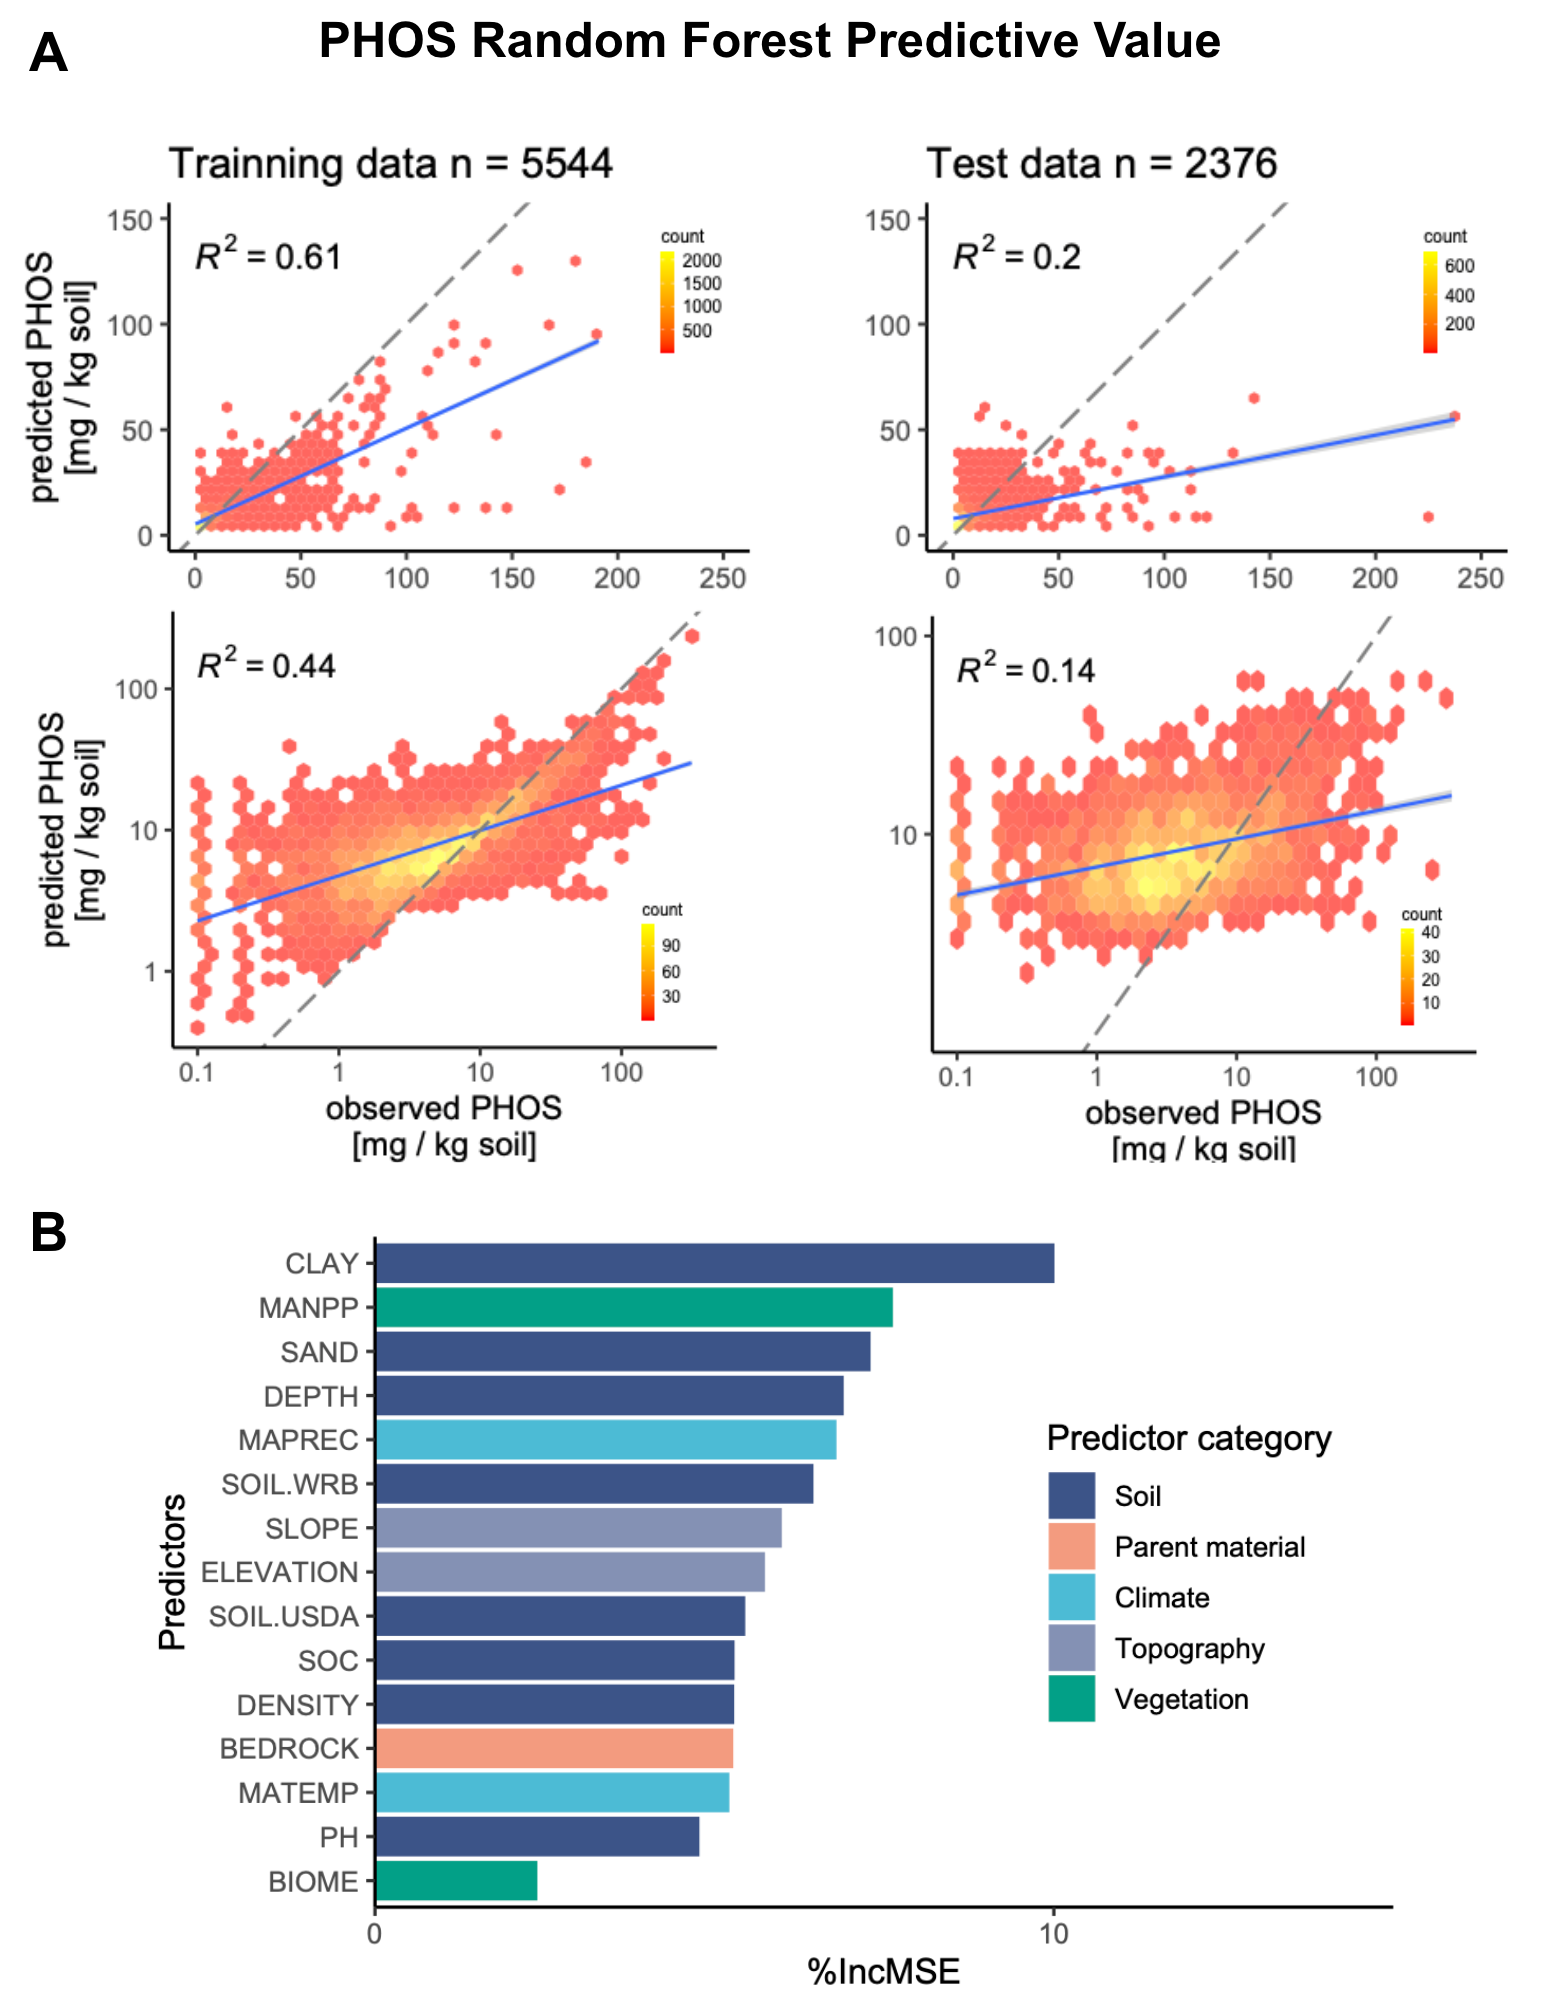
\includegraphics[width=0.9\linewidth]{Chapter-2/figs/rf_validation.png}
\caption[Random forest model validation for soil  available phosphorus PHOS in Mexico]{\textit{\textbf{Random forest model validation for soil  available phosphorus PHOS in Mexico.}}\\\hspace{\textwidth} 
\textbf{(A)} Correlation between observed and predicted available phosphorus in linear (top) and logarithmic (bottom) scales.
The model is overfitted as it has far better predictive value over training $r=0.8$ rather than testing $r=0.4$ data.
\textbf{(B)} Predictor contribution calculated as mean square error difference (\%) after removing it from the model.}
\label{fig::rfvalidation}
\end{figure}
\clearpage





\begin{figure}[!ht]
\centering
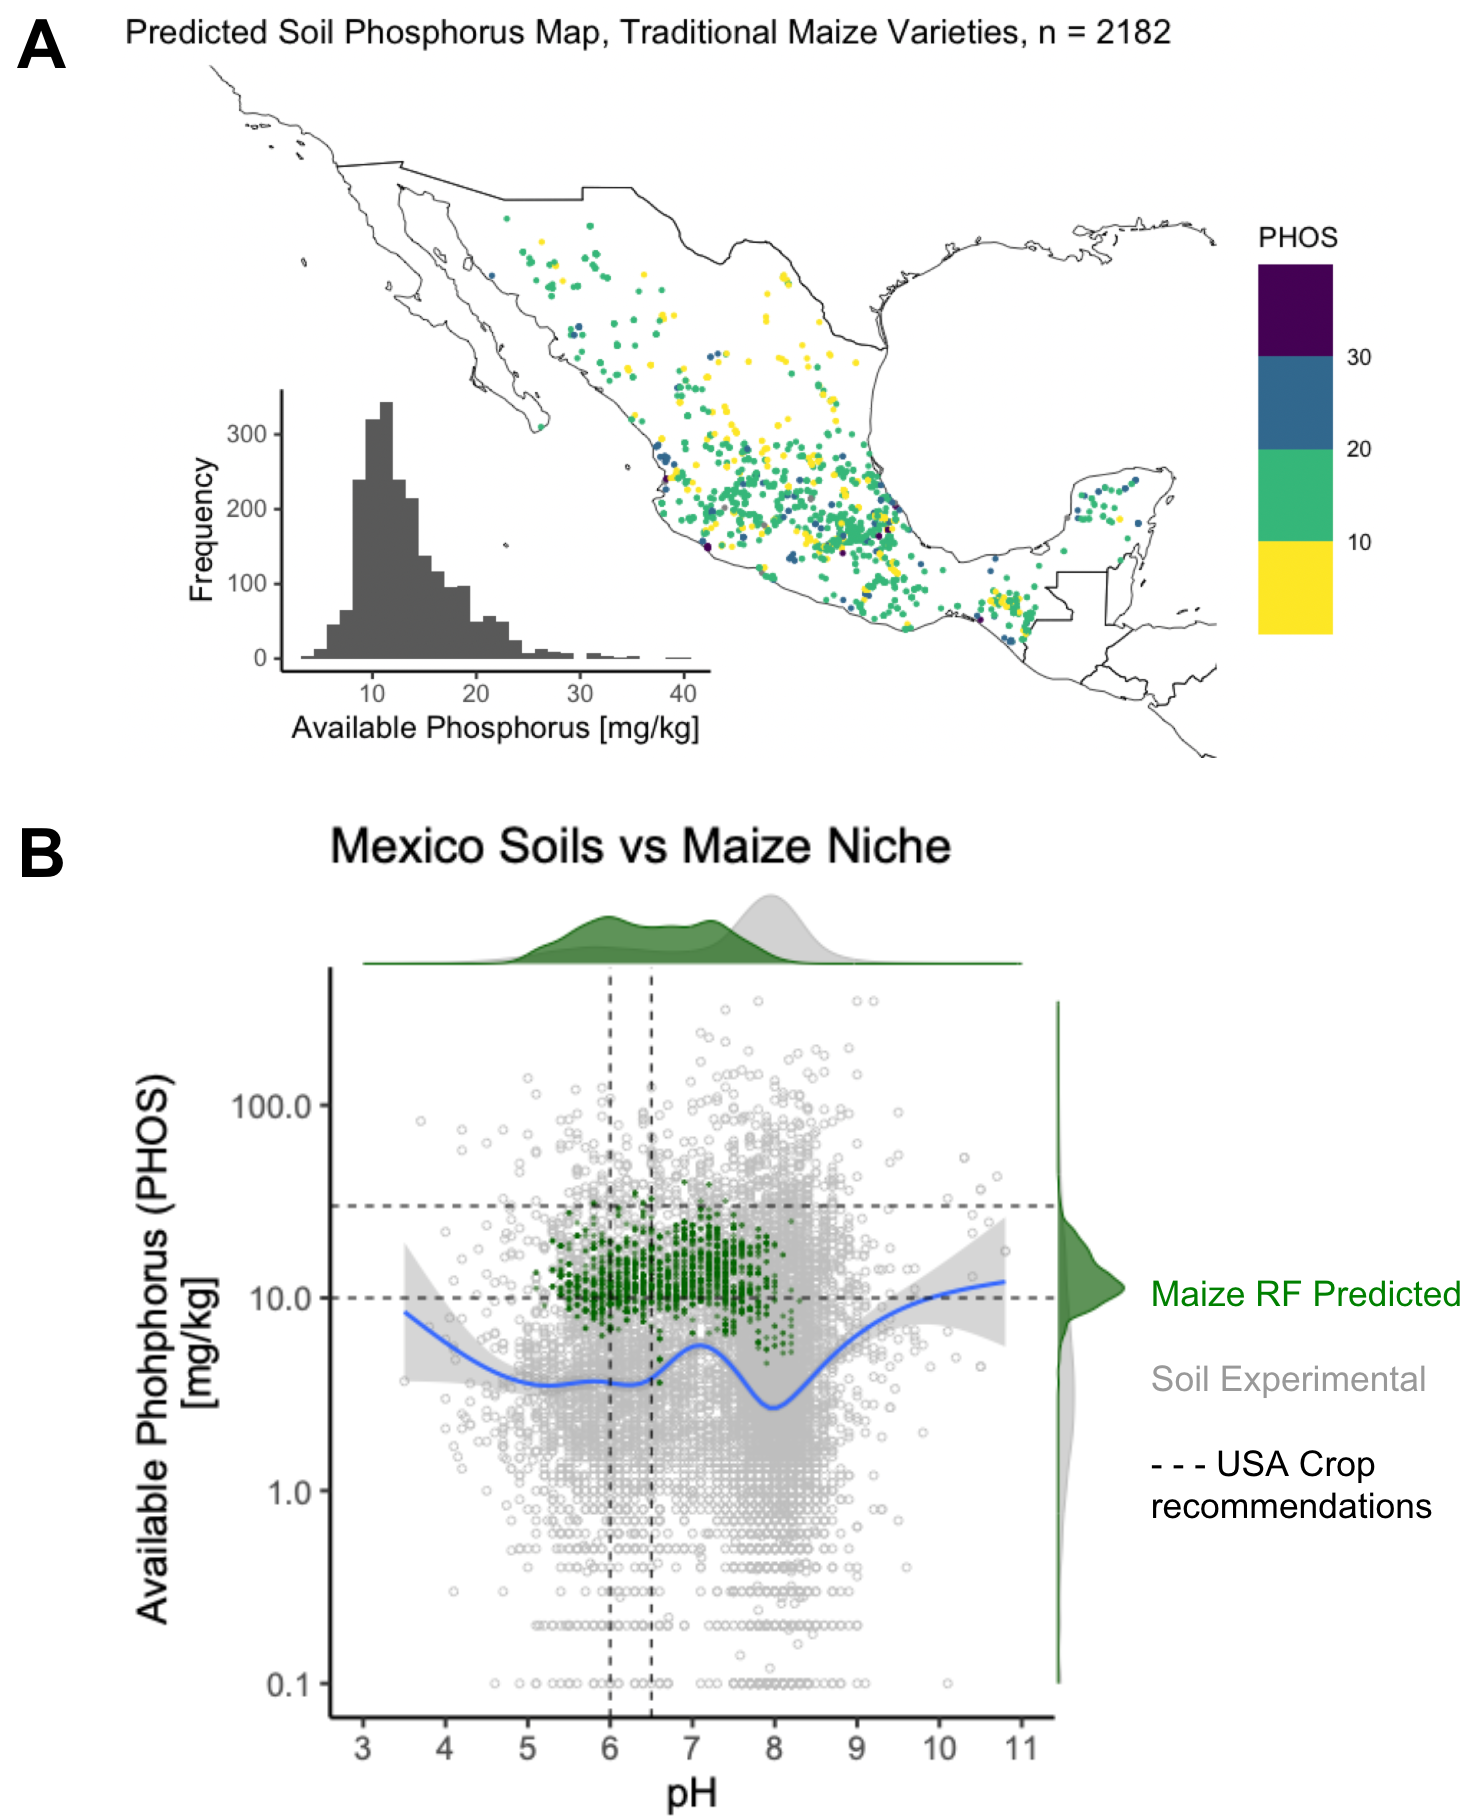
\includegraphics[width=\linewidth]{Chapter-2/figs/predicted_PHOS.png}
\caption[Predicted Available Phosphorus for Mexican Traditional Maize Varieties]{\textit{\textbf{Predicted Available Phosphorus for Mexican Traditional Maize Varieties.}}
\\\hspace{\textwidth}
\textbf{(A)} Geographical distribution for 2182 traditional varieties from the FOAM panel \citep{romero_navarro2017-cn}
\textbf{(B)} Comparison of topsoil phosphorus in 13092 soil profiles \citep{paz-pellat2018} with the predictions for the FOAM panel.}
\label{fig::pointpred}
\end{figure}
\clearpage

\subsection{Genome Environment Associations Point to Candidate Genes for Adaptation to Diverse Soil Phosphorus Availability Conditions}

Now with the best model of plant available phosphorus for Mexican soils  I  proceeded to look for Genome Environment Associations in Traditioal maize varieties in Mexico.

\subsection{Discussion}

% \begin{figure}[b]
% \centering
% 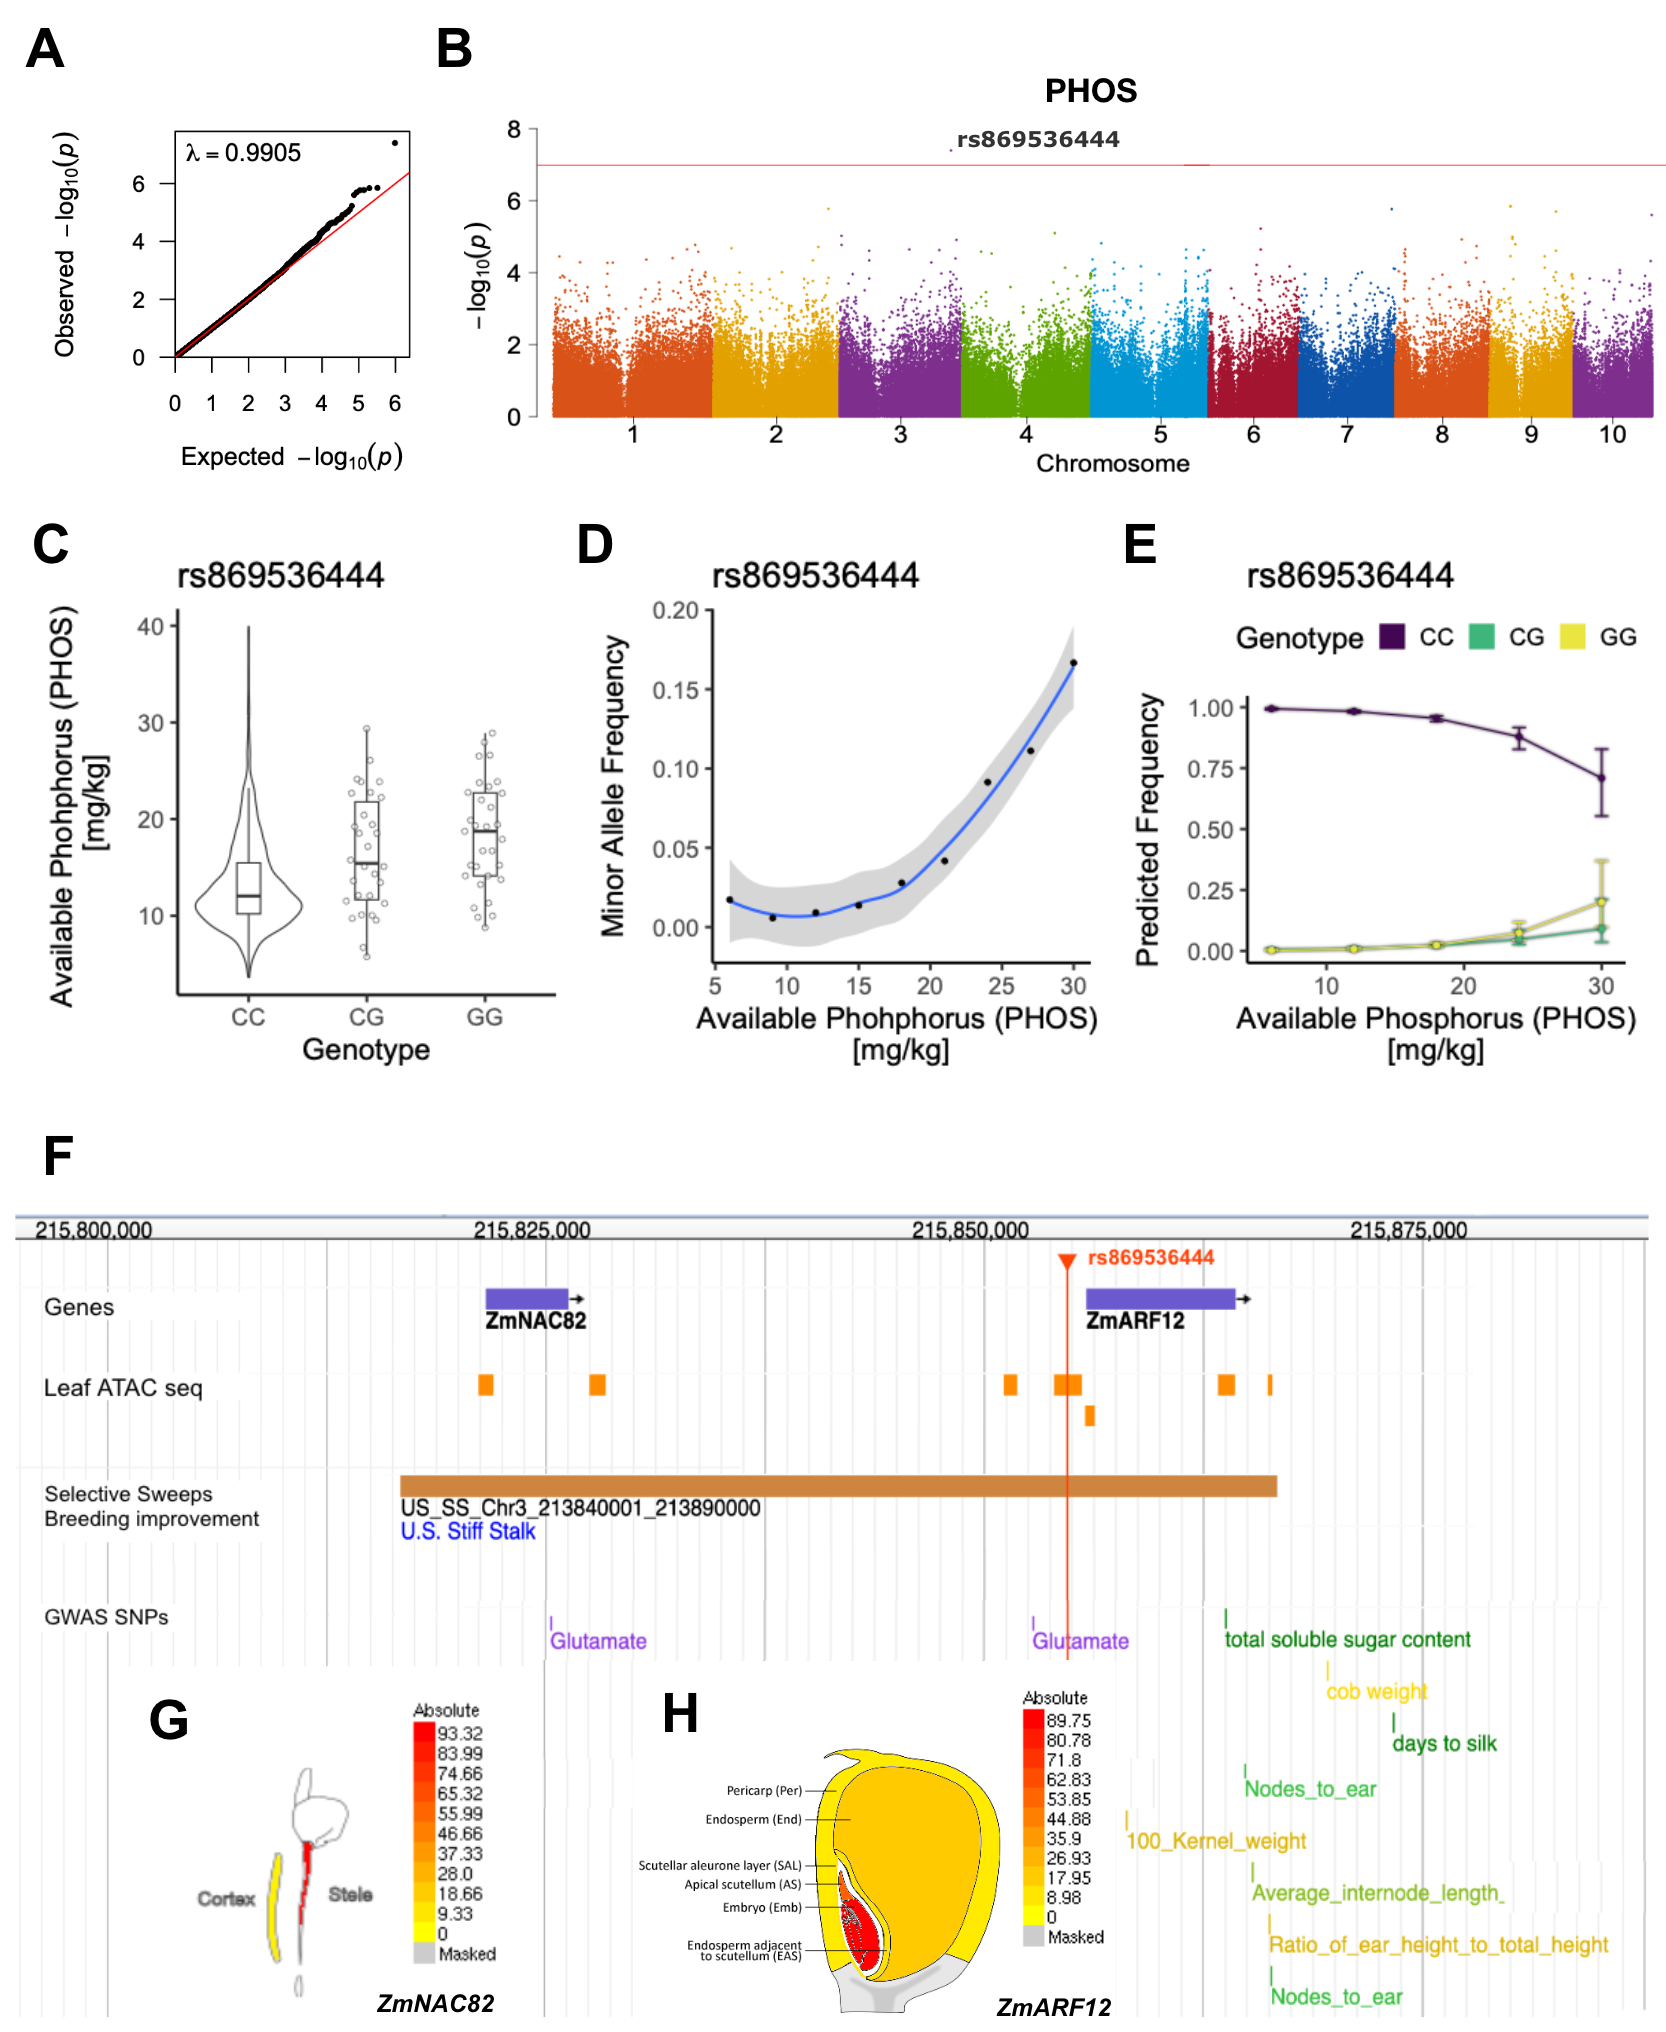
\includegraphics[width=\linewidth]{Chapter-2/figs/PHOS_mlm.png}
% \caption[]{}
% \label{fig:PHOS_mlm}
% \end{figure}
\clearpage

%\addtocounter{figure}{-1}
\begin{figure} [t!]
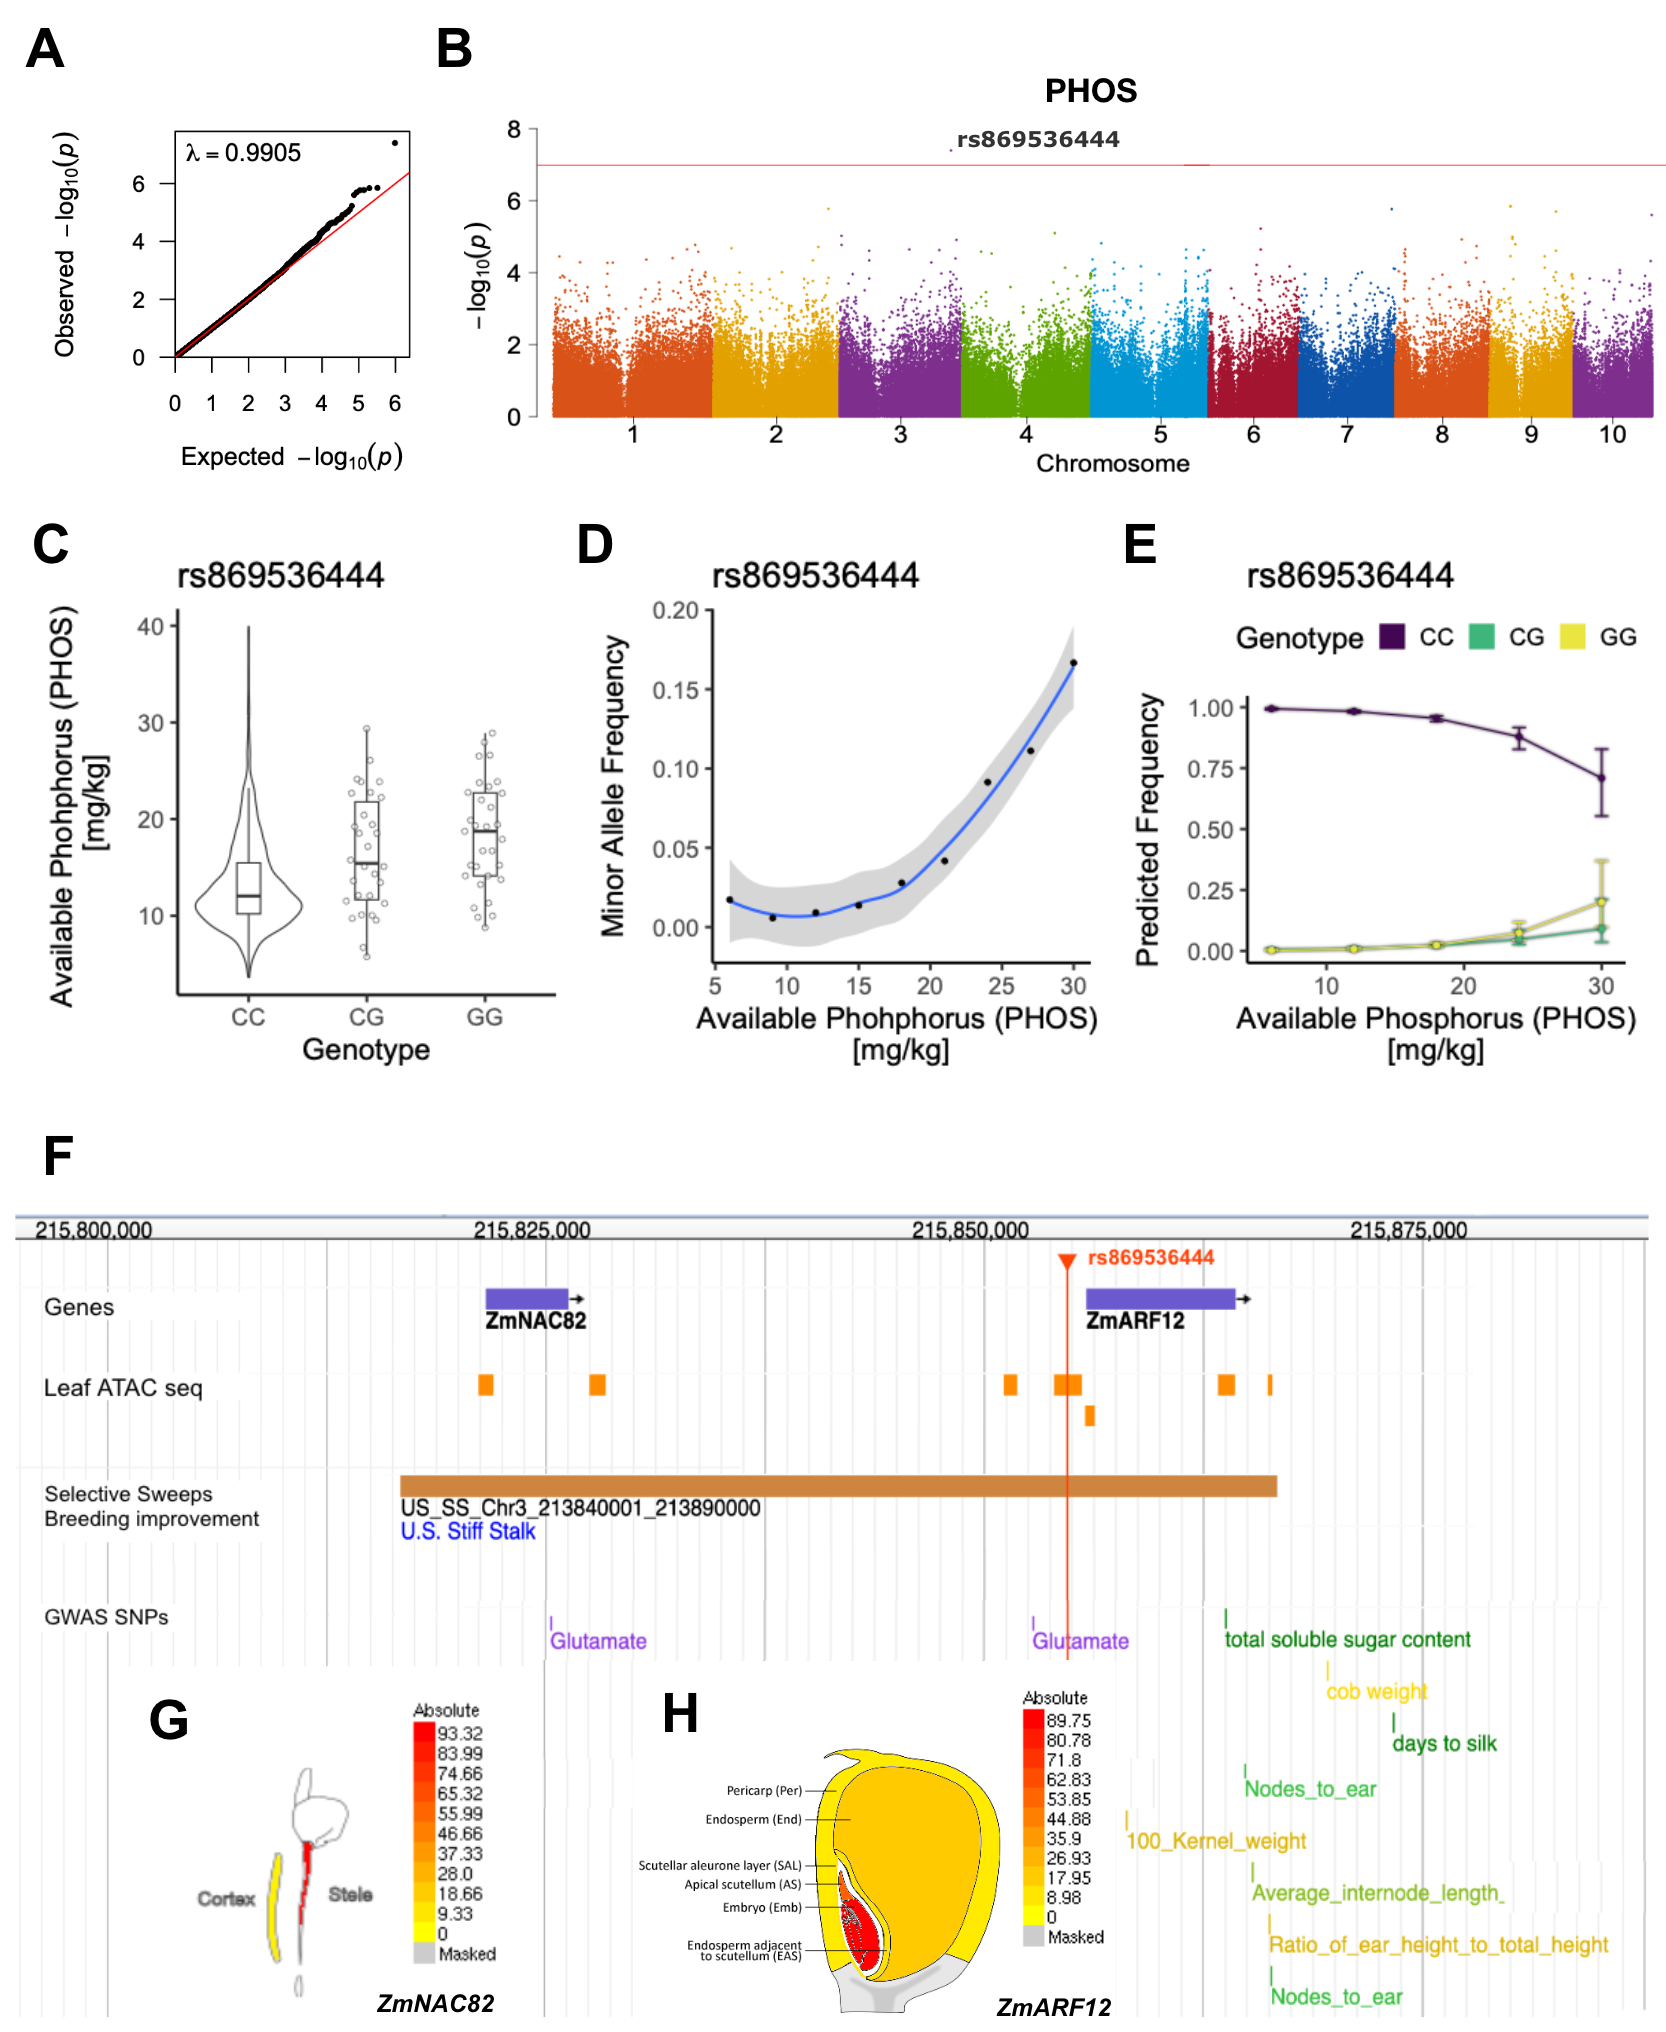
\includegraphics[width=0.8\linewidth]{Chapter-2/figs/PHOS_mlm.png}
\caption[Linear Mixed Model Association between Maize Genetic Variants and Soil Available Phosphorus in Mexican Traditional Varieties]{\textit{\textbf{Linear Mixed Model Association between Maize Genetic Variants and Soil Available Phosphorus in Mexican Traditional Varieties.}}
%% \\\hspace{\textwidth}
\textbf{(A)}  QQ-plot showing genomic inflation factor of p-values of the LMM association
\textbf{(B)} Corresponding Manhattan plot 
\textbf{(C)} Allelic substitution "effect" of rs86953444 on PHOS.
\textbf{(D)} Allele frequency cline.
\textbf{(E)} Multinomial logistic regression of Genotype Frequency on PHOS.
\textbf{(F)} Genomic context of rs86953444 pointing to an auxin response transcription factor candidate \textit{ZmARF12}.
\textbf{(G)} \textit{ZmNAC82} kernel expression.
\textbf{HG)} \textit{ZmARF12} kernel expression.
}
\end{figure}
\clearpage

\begin{figure}[!ht]
\centering
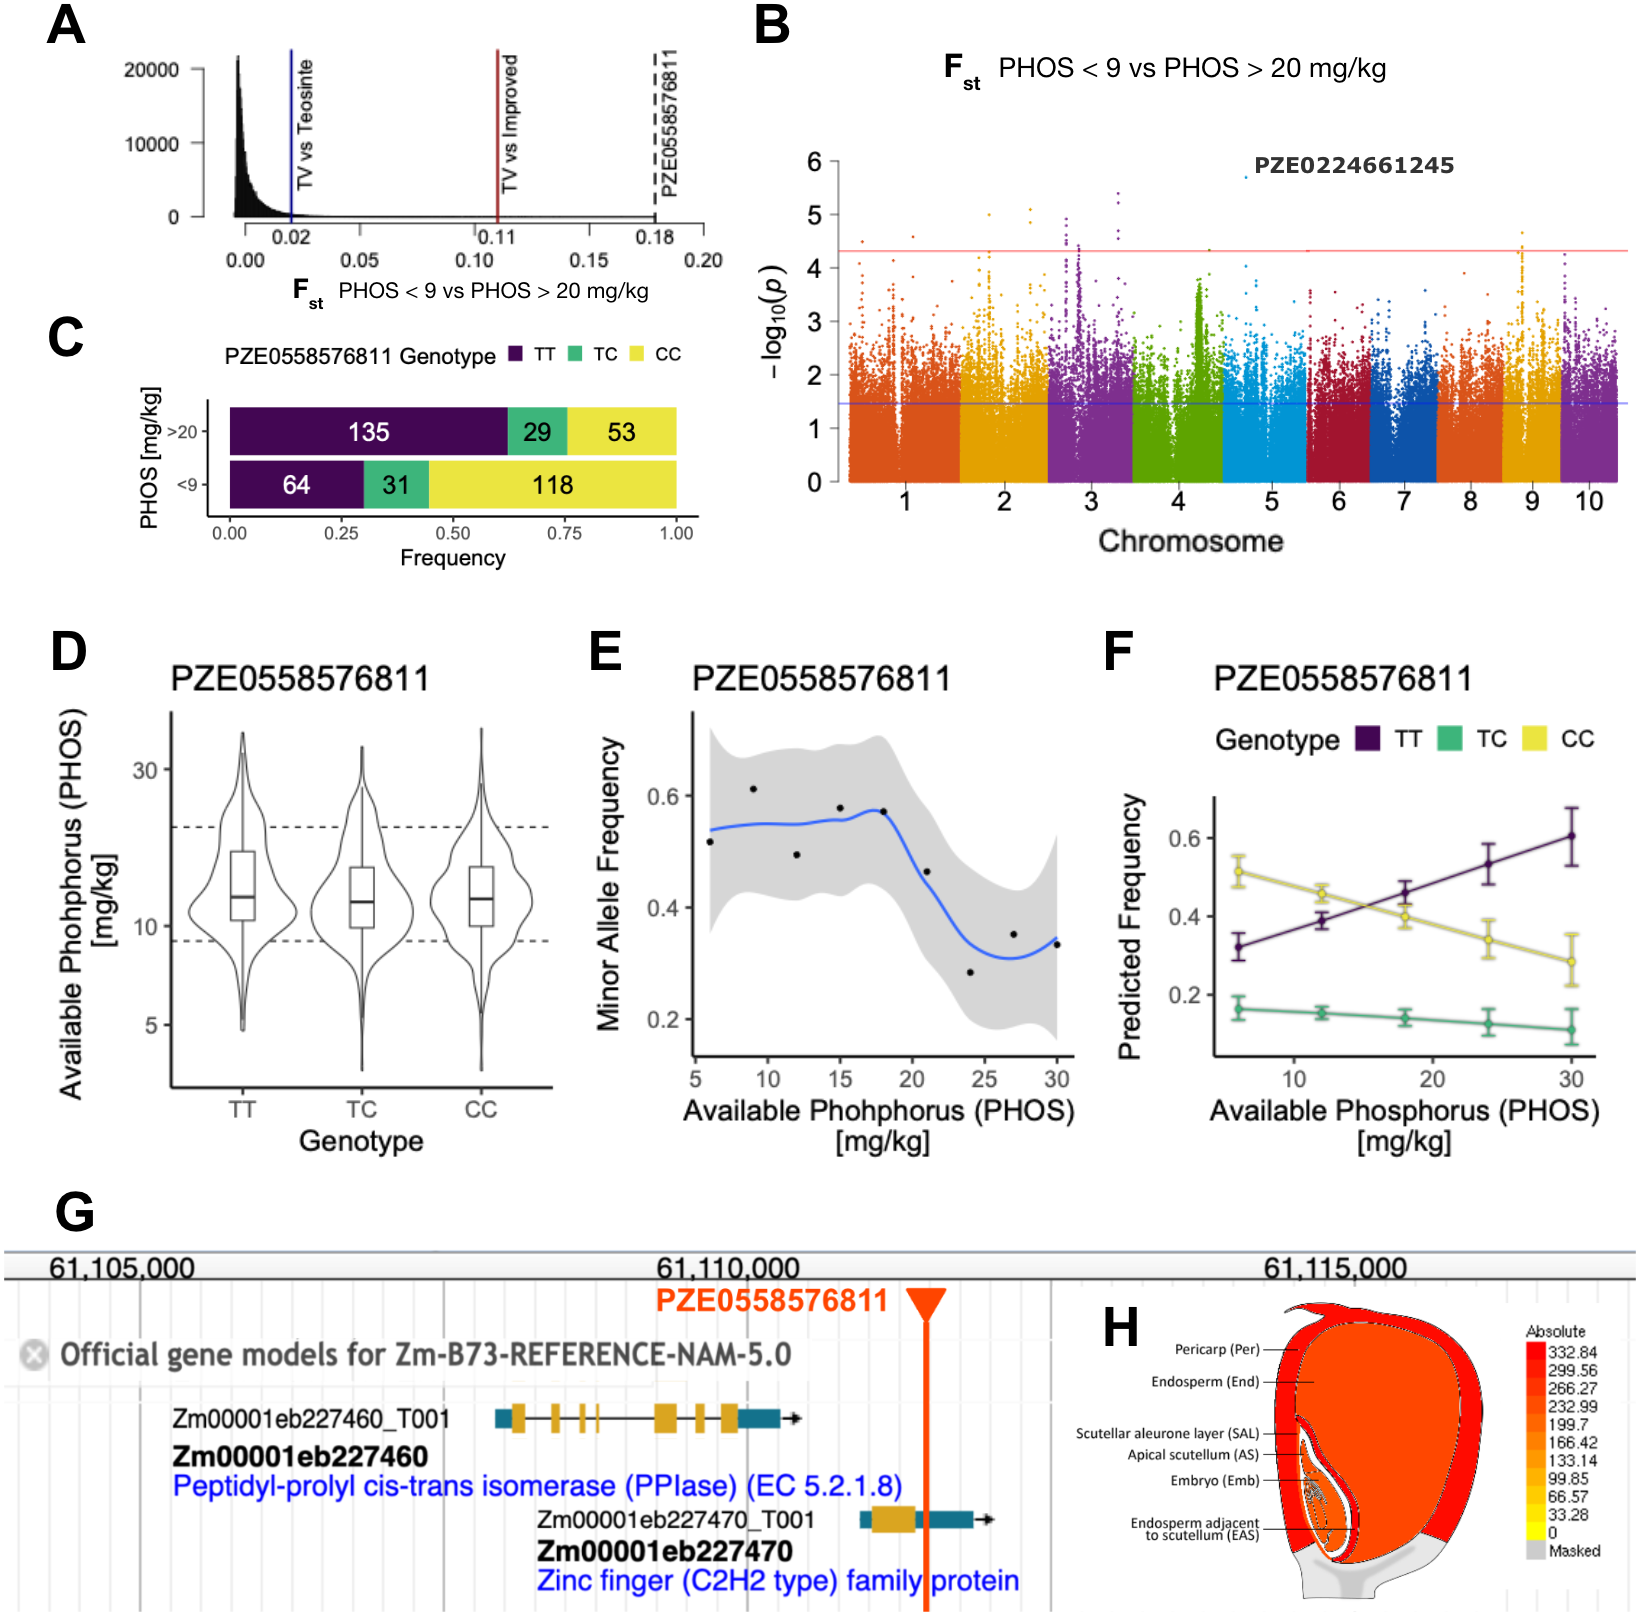
\includegraphics[width=\linewidth]{Chapter-2/figs/PHOS_Fst.png}
\caption[Fst based Association between Maize Genetic Variants and Soil Available Phosphorus in Mexican Traditional Varieties]{\textit{\textbf{ $\boldmath{F_{st}}$ based Association between Maize Genetic Variants and Soil Available Phosphorus in Mexican Traditional Varieties.}}
% \\\hspace{\textwidth} 
\textbf{(A)} Genome $F_\text{st}$ distribution   showing differentiation between extreme deciles of PHOS $<9$ and $>20$ ppm. Three bars are shown for comparison, weighted genomewide mean $F_\text{st}$ \citep{hufford2013-gs} between blue: Mexican maize traditional varieties (TV) and tesosinte (\textit{mexicana} and \textit{parviglumis});  red: TV vs improved germplasm; and dashed: maximum $F_\text{st}$.
\textbf{(B)} Corresponding Manhattan plot.
\textbf{(C)} Genotype frequencies at the SNP with maximal differentiation PZE0558576811
\textbf{(D)} Allelic substitution "effect" on PHOS \textbf{(E)}Allele frequency cline.
\textbf{(F)} Multinomial Logistic Regression of Genotype Frequency on PHOS.
\textbf{(G)} Gneomic contest of PZE0558576811 pointing to a transcription factor candidate  Zm0001eb22747 \textbf{(H)} Zm0001eb22747 kernel expression.
 }
\label{fig::PHOS_Fst}
\end{figure}
\clearpage


\printbibliography[heading=subbibnumbered, title=References]